% siminos/blog/flotsam.tex
% $Author$ $Date$
%
% Predrag moved from thesis/chapters/ back to blog  oct  2 2009
% Predrag moved from blog/ to thesis/chapters/      jun 26 2008
% Predrag created file                              jun 20 2006



% ---------------------------------------------------------------------------
% Removed from lead paragraph by Daniel 04/17/2012. I suggest keeping the lead
% paragraph more general. I think the paragraph flows more smoothly without it.
% We can always talk about the "excellent" methods later.
There exist many excellent methods that quotient out symmetries of
low-dimensional systems, but so far only one, the \mslices, has proven
practical for the extremely high-dimensional flows of turbulent fields.
% ---------------------------------------------------------------------------

\chapter{SCD07 flotsam}

This chapter contains material which has not been included in \emph{On
the state space geometry of the {Kuramoto-Sivashinsky} flow in a periodic
domain}\rf{SCD07}, {\tt siminos/rpo\_ks/} in this repository,  and/or
Siminos Ph.D. thesis\rf{SiminosThesis}. Please clean up whatever seems
extraneous.

\section{Example dynamical systems used throughout this work}
    \label{s:exampleIntro}
% Chapter Introduction, section Example dynamical systems used throughout the thesis.
% $Author$ $Date$
% Label: s:exampleIntro

In this section we briefly introduce some dynamical systems
that will be used as simple examples to demonstrate various
concepts in later chapters.

\paragraph{Lorenz, refchap~{chap:Lorenz}:}
%
\ES{Perhaps say Lorenz flow, complex Lorenz flow etc.}
Lorenz introduced his celebrated equations\rf{lorenz} as a
severe truncation of the Navier-Stokes equations describing
Rayleigh-Benard flow. They read
\index{Lorenz equations}
\begin{align}
\dot{x} &= \sigma (y-x) \notag \\
\dot{y} &= \rho x - y - x z \\
\dot{z} &= x y - b z \notag
\end{align}
where $\sigma$ the Prandtl number, $\rho$ the Rayleigh number
and $b$ an aspect ratio of the problem.

\paragraph{{\CLf}, refchap~{chap:lasers}:}
%
Gibbon and McGuinness\rf{GibMcCLE82} introduced {\CLf}
\beq
\begin{split}
	\dot{x}_1 &= -\sigma x_1 + \sigma y_1\cont
	\dot{x}_2 &= -\sigma x_2 + \sigma y_2\cont
	\dot{y}_1 &= (r_1-z) x_1 - r_2 x_2 -y_1-e y_2 \cont
	\dot{y}_2 &= r_2 x_1 + (r_1-z) x_2 + e y_1- y_2\cont
	\dot{z} &= -b z + x_1 y_1 + x_2 y_2
	\label{eq:introCLeR}
\end{split}
\eeq
as a low-dimensional model of baroclinic instability in the
atmosphere. {\CLf} is equivariant under the action of
$\SOn{2}$.

 \paragraph{\KS, refchap~{chap:KSe}:}
 The \KS\ system
 \beq
   u_t = F(u) = -{\textstyle\frac{1}{2}}(u^2)_x-u_{xx}-u_{xxxx}
     \,,\qquad   x \in [-L/2,L/2]
 \ee{intro:ks}
 was introduced by
 Kuramoto and Tsuzuki\rf{ku} as a phase equation for
 reaction-diffusion systems described by Complex Ginzburg-Landau
 equation and independently by Sivashinsky\rf{siv} to describe
 instabilities in laminar flame fronts.


\section{Squirreled away for the next KS paper}
% from energy.tex

Rescuing back what we squirreled away for the thesis from
material omitted form the KS papers. Predrag moved the
material to thesis from blog/flotsam.tex on June 26 2008, and
back again Oct  2 2009.

\begin{description}
\item[2006-08-20 Lan]
    I checked the equilibria for $L=22,\nu=1$.

Up to now, I only found in the antisymmetric subspace one nontrivial
equilibrium (and its antisymmetric image).

\begin{verbatim}
antfix221.eps 	 projection on (u,u_x) plane
antfix222.eps 	 profile on [0,L]

In our Fourier modes in the antisymmetric phase space, it is
(0.206219058
-0.0460527498
0.10611909
-0.0914948837
0.0289519109
-0.00891853352
0.00416308621
-0.00174073683
0.000569333687
-0.000181945368
6.33396326E-05
-2.17114045E-05
6.98611301E-06
-2.21365123E-06
7.10879216E-07
-2.27150037E-07).
	truncation n=16.

It has an unstable plane with complex unstable eigenvalues
(0.0823534721, 0.340213183), (0.0823534721, -0.340213183).
	PC: period 18.46
	    radial multiplier: 4.5765 = e^{0.08235 2\pi/0.34021}
	    a bit short?

All other eigenvalues are stable:
the next biggest are the complex pair
(-0.228656552, 0.196259159), (-0.228656552, -0.196259159).
	PC: period 32.01
	    radial multiplier: .0006626 = e^{-0.22866 2\pi/0.19626}
	    nicely contracting

Corresponding to the unstable eigenvalues, we have the complex unstable
eigenvectors:
(Re(x),Im(x))= (0.423144666,9.66121118E-09) (-0.249712595,-0.601182048)
(-0.466489695,0.298205956) (0.26189669,-0.0837391834)
(-0.0249213253,0.0961148919) (0.020355046,-0.0604044583)
(-0.0216934611,0.0219640536) (0.00863141624,-0.0077589185)
(-0.00239069432,0.00344187394) (0.000917888558,-0.00142180956)
(-0.000408503874,0.000504218361) (0.000148314512,-0.000174772494)
(-4.82626002E-05,6.30218905E-05) (1.66504428E-05,-2.23354177E-05)
(-5.93090471E-06,7.57642794E-06) (2.01374131E-06,-2.53389912E-06),
whose real part and imaginary part constitute the unstable eigenplane in the
antisymmetric phase space.

Corresponding to the least stable
eigenvalues, we have the complex unstable eigenvectors:
(Re(x),Im(x))= (0.477760491,-1.43027299E-08) (-0.361452174,0.149602413)
(0.341883763,-0.228094857) (-0.361131881,0.482179271)
(0.200427278,-0.184603802) (-0.0790949342,0.0589793411)
(0.0351101345,-0.0321727495) (-0.0162721328,0.0167979654)
(0.00650900391,-0.00620309818) (-0.00236527242,0.00212159114)
(0.000869261277,-0.000809193048) (-0.000321153544,0.000308219102)
(0.00011403128,-0.000107728376) (-3.91786331E-05,3.64500383E-05)
(1.33642382E-05,-1.25202568E-05) (-4.53931493E-06,4.28505972E-06)


\end{verbatim}





\end{description}


{\bf PC}: a bit of a cheat - reffig~{f:KS22unstM} has
    2 unstable complex-pair planes

rescue the nice heteroclinic connection figure
    in reffig~{f:KS22unstM}\,(\textit{b})

    refFig~{f:KS22unstM} move (a) to flotsam

{\bf RLD:} I have the feeling that it can be proven that there are
no other types of symmetries that lead to exactly periodic
solutions, but I don't know how to construct such a proof.
%In the first case the whole orbit lives within the antisymmetric subspace.

\bigskip


{\bf PC} March 2009:
if you really believe that --let's say- B. Hof's pipe is an example of ``chaos,'' more
    power to you. But please do include our referee's precise definitions of
    chaos, spatio-temporal chaos and turbulence in the thesis.

{\bf ES} March 2009: No, I don't consider Hof's pipe to be ``chaos'',
		but do we have a better, widely accepted word
		that describes this Kuramoto-Sivashinsky system? I anyway
		find the definition of ``spatio-temporal chaos'' suggested
		by the referee vague. To me it looks more that it is an issue
		of broken symmetry in \KS\ rather than system size,
		at least that's what I get when I read Manneville's book.
		What I was really trying to
		say is that we call it turbulence because it is not
		what people refer to as chaos. I've dropped both chaotic
		and spatiotemporally chaotic.


{\bf ES} March 2009:
There exist two methods to convert a non-free\ES{but
effective} action of a group $\Group$ on a manifold $\Manif$
to a free action: one either prolongs the action to jet space
and thus calculates differential invariants, or considers the
action of the group in $n$ copies of $\Manif$ with $n>>0$ and
thus calculates joint invariants, see refref~{Olver2000} for
applications. The second method will not be helpful for us
since the dimension of the manifolds that we are interested
in is already very high. We have not found a way to implement
the method of prolongation efficiently for the problems
considered here. The way to get around non-free actions will
be explained in refsect~{laserMFnum}.


{\bf ES} March 2009:
The Gr\"{o}bner basis methods usually perform poorly as $n$
becomes larger than six. On a 1GHz Pentium III processor the
fundamental invariants for $n=16$, for the cross section
$b_1=0$, were computed in approximately 130s. Most
importantly the time was mostly spend in simplification of
expressions.

refFig~{f:ks22rposT}\,(\textit{a}) shows the \rpo s in the plane
$(\period{},\shift)$.  Not much is learned from such plot other than
that for longer periods the \rpo s are scattered over the
whole $(\period{},\shift)$ plane.

The scatter of the largest Floquet exponents
of periodic and \rpo s is shown in reffig~{f:ks22rposT}\,(\textit{b}).
In this case some tendency of accumulation toward the largest
Lyapunov exponent 0.048 of the chaotic attractor
can be noted.  This, however, is in part an artifact of initializing
the \rpo\ searches by near recurrences in long-time \statesp\
trajectories.


\subsection{Template for KS \eqva\ discussion}

\noindent
{\bf 2006-09-03 Ruslan}
KS \eqva\ discussion:
\\
\HREF{http://www.math.le.ac.uk/people/rld8/temp/kse22explore.html}
{www.math.le.ac.uk/people/rld8/temp/kse22explore.html}

{\bf ES:}{I observe pairs of real eigenvalues,
e.g. -58.3602685 and -58.3602681. As their absolute
value increases they differ even less.
I think it has to do with the linear part being the main
contribution to $\Mvar$ for higher modes, as well as
with treating real and imaginary components
as separate variables, which means it will appear twice.
        }

PC: {I think such contracting eigenvalues as -58.3602685 have no meaning.
Even if they are accurate eigenvalues of $\Mvar$,
what use is
$\ExpaEig_{radial} =  e^{\Lyap_p \period{p}} = e^{26\cdot58} = e^{1510}$.
        }

The \reqva\ (or traveling waves) appear to have a limiting propagation
velocity $c_{max} = \pm d/\period{}$.
To visualize them numerically,
start with a localized self-dual $u(x,0)$ such as
\[
u(x,0) = x e^{- x^2/2\sigma^2}
\,,
\]
with typical width $\sigma/2$ of order of typical wavelength
$\sqrt{2}$ (in $\tilde{L}$ system size units).
Time evolution of this  $u(x,t)$ is bracketed by two constant
pulses of apparently constant velocity $v=?$.
\RLD{generate figure, state $\sigma/2$, estimate $v$}
The notion of ``velocity''
is fuzzed up by the fact that the large peaks are preceded
by smaller precursors.

PC: {Determine their velocity ANALYTICALLY?}

we have to systematize it, and
construct the complete cage of heteroclinic $\EQV{1}$, $\EQV{2}$, $\EQV{3}$,
$\REQV{+}{1}$,
$\REQV{-}{1}$,(?)
connections, \underline{divided} by the $u(x) \to - u(-x)$ symmetry.

The hope is that $\EQV{1}$,
$\REQV{+}{1}$,
$\REQV{-}{1}$,(?) are transient, and \rpo\ symbolic
dynamics (\underline{divided} by the $u(x) \to - u(-x)$ symmetry, otherwise
unnecessarily messy) comes from the closed loops on
the $\EQV{2}$,$\EQV{3}$ part of the cage.



{\bf example - Stability of \KS\ \eqva:}{
% \label{exam:KSEquilStab}
% \index{Kuramoto-Sivashinsky equilibria}
\begin{table}
\caption[Important \KS\ equilibria]{
Important \KS\ \eqva:
% in the antisymmetric solution
% space of the \KSe\ with periodic boundary % % % % condition,
% $ \nu =1$, $L=38.5$;
% their labels,
the first few stability exponents
%, with complex pairs written together.
}
\begin{center} \footnotesize
\begin{tabular}{@{}ccccc}
\hline %\br
$~S~~~$ & $~~~~\lambda_1 \pm \,i\,\theta_1$
                                & $~~~~\lambda_2 \pm \,i\,\theta_2$
                                        & $~~~~\lambda_3 \pm \,i\,\theta_3$
\\
\hline %\mr
${C_1}$    &{0.04422 $\pm \,i\,$0.26160}   &-0.255 $\pm \,i\,$0.431
&-0.347 $\pm \,i\,$0.463         \\
% ${C_2}$    &0.33053  & 0.097 $\pm \,i\,$0.243
% &-0.101 $\pm \,i\,$0.233        \\
\hline %\mr
${R_1}$   &{0.01135 $\pm \,i\,$0.79651} & -0.215 $\pm \,i\,$0.549
&-0.358 $\pm \,i\,$0.262        \\
%  ${R_2}$   &  0.33223  & -0.001 $\pm \,i\,$0.703
%  & -0.281 $\pm \,i\,$0.399      \\
\hline %\mr
${T}$     & 0.25480  & -0.07 $\pm \,i\,$0.645 &-0.264
\\
\hline %\br
\end{tabular}
\end{center}
\label{t:stationary}
\end{table}

{\em
spiraling out in a plane}, all other directions contracting


{\bf
Stability of ``center'' \eqv\
    }

linearized stability exponents:
\[ % \beq
(\lambda_{1}\pm\,i\,\theta_{1},\lambda_{2} \pm\,i\,\theta_{2}, \cdots)
    = (0.044 \pm \,i\,0.262\,,\,
        -0.255 \pm \,i\,0.431\,,\,\cdots)
\] %\eeq

The plane spanned by $\lambda_{1} \pm\,i\,\theta_{1}$ eigenvectors rotates with angular period
$\period{} ~\approx~2\pi/\theta_{1}=24.02$.
% 2*4*a(1)/0.26160 = 24.0182924586375

a trajectory
that starts near  the $C_1$~\eqv\ point spirals
away per one rotation
with multiplier
$\ExpaEig_{\mbox{radial}}~\approx~\exp(\lambda_{1}\period{})=2.9$.
% 2*4*a(1)/0.26160*0.04422 = 1.062
% e(1.0620888) = 2.8924063421

each Poincar\' e section return,
contracted into the stable manifold by
factor of
{
$\ExpaEig_{2}\approx\exp(\lambda_{2}\period{})=0.002$
}
%2*4*a(1)/0.26160*(-0.255) = -6.12466
%e(-6.12) = .0022


The local Poincar\' e return map is
{\em
in practice $1-dimensional$
}
    } %end \example{{Stability \KS\ equilibria


Staring at the solution
 as it evolves in time we should start getting a glimpse of the
 repertoire of the spatiotemporal patterns characterizing
 the turbulent dynamics.

Many of the \rpo s can be constructed from segments corresponding to
close approaches to some of these \eqva.

\textbf{ES}: Greene and Kim show that steady states (non-traveling)
have to be antisymmetric and our findings verify it.

\textbf{PC}: do they really show that? I think they must be symmetric under both
{\Refl} and \Shift, otherwise they could be invariant under one,
but traveling, not invariant under the other one.

\textbf{ES}: They provide an argument for this which did not yet convinced me.
\EQV{2,3} are symmetric under both {\Refl} and \Shift, \EQV{1} is not
symmetric under \Shift, but when I say traveling I mean traveling waves,
this does not refer to behavior under symmetry.

If Greene and Kim
are correct we would get the same \eqva\ for both
antisymmetric and full space. If \eqva\ provide the coarsest organization
of \statesp\ then we should expect characteristic orbits for $L=22.0$
for full space and $L=44.0$ for antisymmetric subspace to be completely different.
Of course for $L=22.0$ the full space dynamics will be richer than
in the
antisymmetric subspace, but I don't think this can be quantified by
dividing $\tildeL$ by $2$.

\textbf{PC}: you are right.


\subsection{Numerical methods}

%% Davidchack and Crofts
 We investigate this system in 16 to 64 complex Fourier modes (32 to
128-dimensional system of real ODEs) truncation, and recheck the results
by redoing the calculation with the double number of Fourier modes. %
observe how many digits change. The \eqv\ points are accurate to at least
to $10^{-11}$. Since Lapack is also double precision accurate, the
accuracy of the first few eigenvalues is similar, and certainly in excess
of 6 significant digits. % All digits stated in tables are significant.
The accuracy that can be reached is of order of
$|a(\period{p},d_p) - a_0|
 \approx \epsilon \exp(\Lyap_p \period{p})$,
 where $\epsilon \approx 10^{-17}$ for double precision, $\Lyap_p$ is
the largest Lyapunov exponent, and $\period{p}$ the period.  With a good
starting guess, Newton's method typically reaches that accuracy after 2-3
iterates.



\subsection{Antisymmetric subspace}
%\label{s:AntisymmSubspFlot}


Perhaps there is some way of plotting the unstable manifolds too. If
there is only one unstable direction (in the full Fourier space
representation), the corresponding eigenvector is a unique loop function
$h[s] =  h(u(s),v(s),w(s))$ in the $(u,v,w)$ space, and the unstable manifold
$U$ is swept out by evolving in time the perturbed loop
$L[s] + \delta h[s] =  L(u(s),v(s),w(s)) + \delta h(u,v,w)$
$\to$ $L[s,t]$.
Complex eigenvector defined unstable manifold plane seems
harder to visualize;  It would be interesting
to look at heteroclinic connections in the $(u,v,w)$ space, as
behavior of higher-frequency modes in Fourier reps is a bit
hard to get used to.

\bigskip

The \KSe\ in  form \refeq{ks} is used, among others, in
\refrefs{cross93,Mks86,ks04com}.

\bigskip

In the Fourier representation they satisfy
the \eqv\ condition for \refeq{expan}
\beq
\left( \frac{k^2}{\tildeL^2} - \frac{k^4}{\tildeL^4}  \right)\, a_k
    \PCedit{
    -  \frac{i k}{2\tildeL} \sum_{m=-\infty}^{+\infty} a_m a_{k-m}
            }
  = 0
\,.
\label{eq:stfks}
\eeq

\bigskip

There appears to be a heteroclinic connection from \EQV{2}
{\eqv} unstable spiral out straight into \EQV{3}~{\eqv}
$\period{} = 76.6$ \rpo\ seems like a close-by relative of
this. That also means that the relative shift between the two
{\eqva} is fixed, as far as this connection is concerned.

% "Ruslan L. Davidchack  2 Nov 2006
%
Isn't there another $ \EQV{2} \to \EQV{3} $ heteroclinic from
the same point on  \EQV{2} circle that connects to a different
point on \EQV{3} circle?
	%
\PC{refFig~{f:KS22rpo} goes to Vaggelis thesis - removed it from the paper,
    as the color schme is different from Ruslan's
   }

\bigskip


%%%%%%%%%%%%%%%%%%%%%%%%%%%%%%%%%%%%%%%%%%%%%%%%%%%%%%%%%%%%%%%%
\begin{figure}[t] \label{f:KS22rpo}
\begin{center}
(a)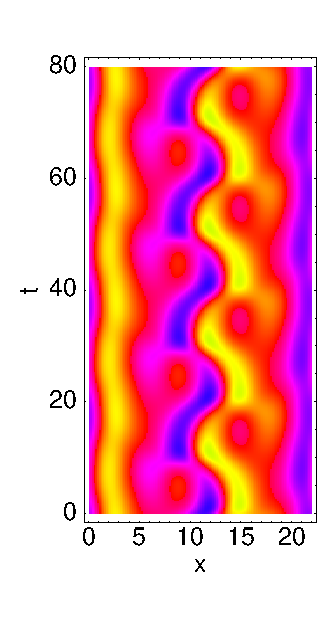
\includegraphics[width=0.2\textwidth]{rpoKS21}
(b)\includegraphics[width=0.2\textwidth]%,origin=c]
                {rpoKS33}
(c)\includegraphics[width=0.2\textwidth]%,origin=c]%
        {rpoKS46}
(d)\includegraphics[width=0.2\textwidth]%,origin=c]%
        {rpoKS56}
\end{center}
\caption[\Rpo s of KS equation]
        {
\Rpo s of KS
equation:
% for $\tilde{L}=3.5014$, N=64 mode truncation.
(a) T=20.51, d=0.0 (\po),
(b) T=32.80, d=10.96,
(c) T=46.51, d=7.76,
(d) T=55.60, d=-5.25.
        }
\end{figure}
%%%%%%%%%%%%%%%%%%%%%%%%%%%%%%%%%%%%%%%%%%%%%%%%%%%%%%%%%%%%%%%%%%

It is imperative that we start using the discrete symmetries, and only 1/2
of trajectory when it is selfdual.
\EQV{1}, \EQV{2} and \EQV{3} and unstable eigenvectors
we care about all happen to sit in the antisymmetric subspace
(recheck...), so connections should reflect these multiplicities. We have
one $\EQV{2} \to \EQV{3}$ and $\EQV{2} \to \EQV{2}$ (shift by $L/4$).

The \rpo\ {\nameit}55 travels between the 2-\eqv\  and
2-\eqv\ shifted,
with period and shift
$\period{p}=55.5953\,,\ d=5.24725$
Compared to $L/4 = 5.5$
this is nice, but why not close to periodic after 2nd return? Why 4th return?

The {\nameit}2 {\eqv}
captures qualitatively the mean velocity frame \rpo\ {\nameit}55 shape,
which follows the
{\eqv} for most of the time, except for a quick swing where it
sidesteps by $d/4$, just as it does in reffig~{f:rpo55}.

\Rpo\ {\nameit}55 looks similar to Davidchack's  orbit
of period
$\period{p}=47.64$ and $d=5.6759$. The period appears to depend on how
many times the orbit manages to spiral around the \eqv.
For {\nameit}55 that appears to be
1.5 times per period, rather than 2. This would led as
to
think there is a family of \rpo s along with a 3rd unit eigenvalue of
$gJ$,
but such does not exist.
So there has to be a selection mechanism corresponding to
reaching or missing the neighborhood of an \eqv\  point starting from
the neighborhood of the other.

The $u$ space time evolution reffig~{f:rpo55u} % rpo22-55-4-u
is plotted with the same starting instant,
so one can also track also the spatial profile $u$ in parallel with
the Fourier space projections.

So it is almost impossible to see reffig~{f:rpo55}(b) %rpo22-55-4-cm
in reffig~{f:rpo55}(a) % rpo22-55-4.
I can see 4 periods in reffig~{f:rpo55}(a), %po22-55-4,
but not in reffig~{f:rpo55}(b) %rpo22-55-4-cm
where it comes back only after full period $\period{p}=55.6$.

It still seems that it could be made relative periodic
(modulo a reflection symmetry?)
in $\period{p}/4=55.6/4=13.9$? That would be OK
-
by symmetry the figure 8 connecting
2 symmetric {\eqva} could consist of 4 identical segments: from
{\eqv} A to midplane, then reflected version of the same to SA, and
back again.

The two {\eqva}
capture qualitatively the mean velocity frame \rpo\ {\nameit}55 shape,
which follows the
{\eqv} for most of the time, except for a quick swing where it
sidesteps by $d/4$, just as it does in reffig~{f:rpo55}.

Please also plot it in plane, chose small Fourier coefficients
 which respect the $x \to -x$ symmetry of \KSe.
Then the symmetry of 2 mean velocity
{\eqva} and self-dual symmetry of \rpo\ {\nameit}55 will be explicit.

Eigenvalues of \rpo\ {\nameit}55 $g\jMps$: are
\\
$(-57.17,  1, 1, -0.500, -0.012, \cdots)$ .
%
%  Eigenvalues of the Jacobian without rotation
%  84.15, -33.86 + 28.94 i, c.c. , 0.48, 0.00019
% no good - missing marginal ones

plots:
  76 rpo60fm23.jpg  \\
 909 rpo60fm23.emf  \\
% Ruslan L Davidchack,  10 Jul 2006
the 55 rpo, or whichever seems easiest to explain:
$\period{} = 59.89$,
$c_p = \shift_p/\period{p}= ?$

$(\ExpaEig_i e^{\pm i\theta_i})=
(
\\
 -27.03397007874626,
\\
   9.34426620337976,
\\
   1
\\
   1
\\
  -0.05018967056231,
\\
   0.00015065158255,
)$

The eigenvectors
indicate that an amplitude mode comes paired with the
group shift-invariant mode $\ExpaEig_4 =1$. It probably says that
the amplitude $|u_k|$ of the associated can be easily perturbed (think of
a large system: $|u(x)|$ can be easily deformed by long wavelength
perturbations. This \underline{must} be understood. Proposal:

There are two
marginal eigenvalues, one for time translation, one for
rotational invariance.
The sign of $\ExpaEig_{1}=-57$ says this is a Moebius-kind orbit,
inverse hyperbolic.
Stability exponent
 $\eigExp[1]=0.07$ says that this neighborhood is much less repelling than
the central {\eqv} A, a better candidate for being embedded into the
ergodic attractor.

The \rpo\ initial condition is
so accurate the orbit in reffig~{f:rpo55}(b)
start visibly deviating after retracing the loop 6.5 times.
% the largest unstable multiplier is
% $-57.17$ per period of the orbit - error would grow to $\approx 60^7
% = 2,800,000,000,000$.

For a numerical check of the \rpo\ stability eigenvalues,
used two inital
points along an unstable eigenvector $\jEigvec{1}$
at radial distance  $\approx 10^{-4}$ from the \eqv\ {\nameit}2,
and the initial inter-point separation $\Delta(0) \approx 10^{-5}$.
Integrated for time equal to the period $\period{p}=26.3556$ as calculated from
the \jacobianM\ and computed the leading Lyapunov exponent from the ratio of
final to initial distance
$\Lyap= \frac{1 }{ \period{}}\ln( \Delta(\period{})/\Delta(0))$.
Get
$\Delta(\period{})/\Delta(0) =39.01$,
$\Lyap=0.13902$, in agreement with the \eqv\ {\nameit}2
expanding eigenvalue $\Lyap=0.13904$
\[
\ExpaEig_{radial} =  e^{\Lyap \period{}} =38.99
\,.
\]

% Ruslan L Davidchack,  10 Jul 2006
The orbit RLD found has period 60
rather than 55.  Because it comes so close to the steady states,
this is probably a numerical precision error.
\\
plots:
 180 rpos1.jpg  \\
1594 rpos1.emf  \\


Rewrite Fourier modes as $u_k(t) = e^{r_k(t) + k(\theta_k(t))}$, study
dynamics and Jacobins in the $\dot{r_k},\dot{\theta_k})$ representation.
\nameit 2 and \nameit 3 \eqva\ are nearly circles in this representation - higher
modes will not wind wildly if represented by $\theta_k(t)$? Kind of WKB
representation.

period 77 rpo jumps between the two steady states.
\\
plots:  \\
  84 rpo77fm23.jpg  \\
1133 rpo77fm23.emf  \\
 176 rpos2.jpg  \\
1594 rpos2.emf  \\


\bigskip

%%%%%%%%%%%%%%%%%%%%%%%%%%%%%%%%%%%%%%%%%%%%%%%%%%%%%%%%%%%%%%%%
\begin{figure}[t]
\begin{center}
(a) 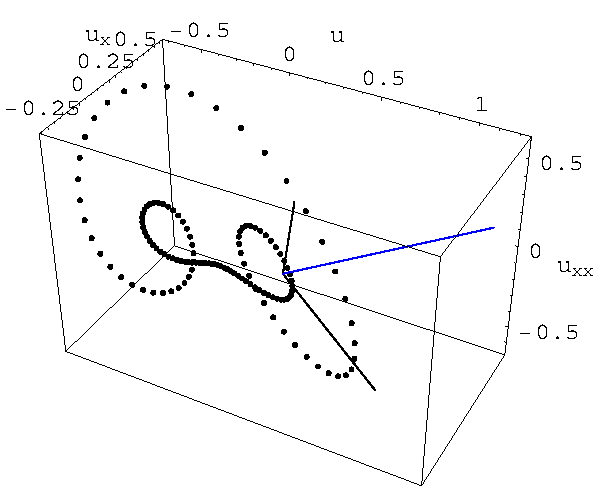
\includegraphics[width=5.0cm]{1wSteadyE}
\hspace{0.1in}
(b) 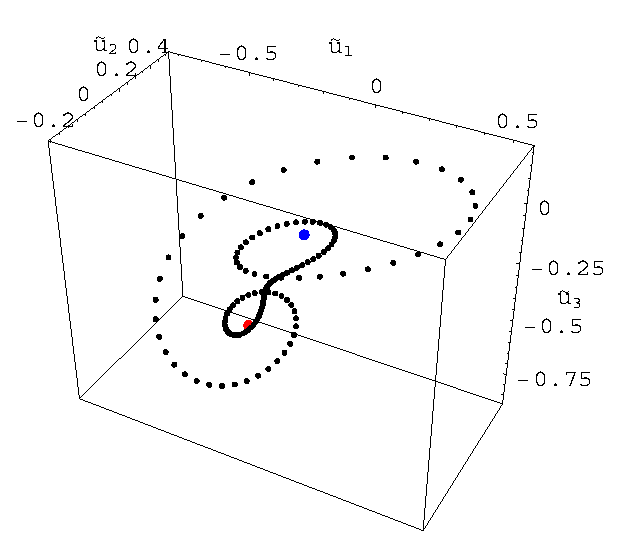
\includegraphics[width=5.0cm]{1wSteadyP}
\end{center}
\caption[EQV{1} visualization]
        {
(a) \EQV{1} in $(u,u_x,u_{xx})$ representation along with the eigenvectors of the \eqv\
point $(\sqrt{c},0,0)$. The blue line represents the unstable eigen-direction.
(b) \EQV{1} projected along the above eigenvectors.
% $\tildeL=3.5014$, $N=64$ complex modes truncation.
        }
\label{f:1wSteady}
\end{figure}


%%%%%%%%%%%%%%%%%%%%%%%%%%%%%%%%%%%%%%%%%%%%%%%%%%%%%%%%%%%%%%%%
\begin{figure}[t]
\begin{center}
    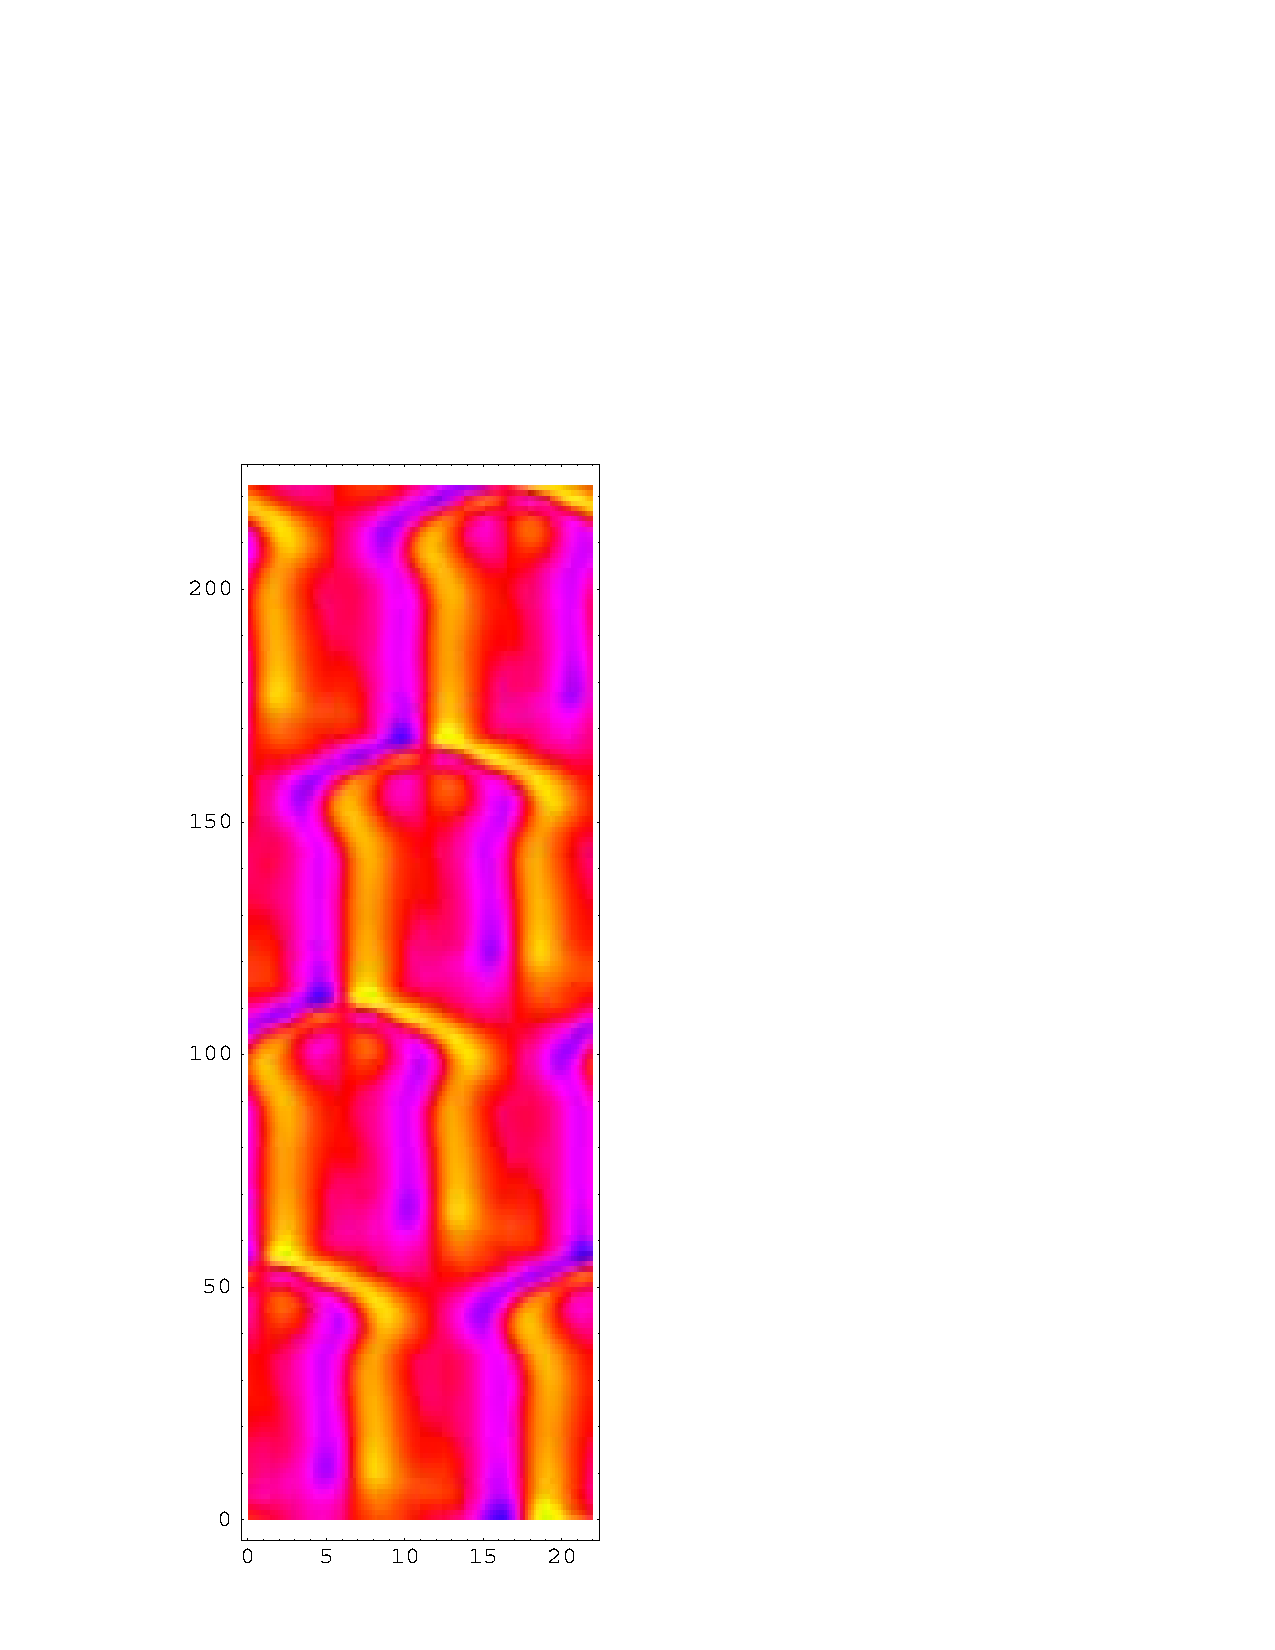
\includegraphics[width=0.18\textwidth]{rpo22-55-4-u}
\end{center}
\caption[The \rpo\ T=55 in  u(x,t)  representation]
        {
 The \rpo\ {\nameit}55 in $u(x,t)$ representation.
        }
\label{f:rpo55u}
\end{figure}
%%%%%%%%%%%%%%%%%%%%%%%%%%%%%%%%%%%%%%%%%%%%%%%%%%%%%%%%%%%%%%%%%%




This observation can be heuristically motivated as follows.
\PC{this argument keeps worrying me: there are lots of solutions, like
$u=0$, that are {\eqva}, but isolated -
they are no place near asymptotic dynamics.
Do they belong to the invariant manifold?
   }
\Eqva\ are solutions valid for all times, and are thus points
on the finite-dimensional compact inertial manifold\rf{infdymnon}.
Finite dimensionality of the inertial manifold
bounds the size of Fourier components of all solutions.
This
compact inertial manifold and the dynamics on it can be
described by analytic functions of a finite number of Fourier modes.
\PC{explain the theory; say that in practice it is useless}
On a finite-dimensional compact manifold,
an analytic function can only have a finite number
of zeros. So the {\eqva}, {\ie},
the zeros of a smooth velocity field on
the inertial manifold, are finitely many.
The number of {\eqva} increases exponentially with $L$,
\PC{give reference for ``exponential growth''}
for infinite system size $L \to \infty$,
there are infinitely many {\eqva}.
\PC{is there a reference where this is explained?}

\bigskip

To illustrate the rapid contraction in the non-leading eigendirections
we plot  in [MAYBE INCLUDE] % reffig~{f:eigenvalues}
the eigenvalues of the \eqv\ in the unstable regime,
for relatively small system size, % low viscosity $\nu$,
and compare them with the
stability eigenvalues of the least unstable cycle for the same
system size.
The `laminar' \EQV{0}~\eqv\ is very unstable,
with many unstable eigendirections.


\bigskip

Even though our starting point \refeq{ks} is an infinite-dimensional
dynamical system, the asymptotic dynamics unfolds on a
finite-dimensional attracting manifold, and so we are back on the
familiar territory: the theory of a finite number of ODEs applies to
this infinite-dimensional PDE as well.

\bigskip

It is very unlikely that a single 1-$d$ Poincar\'e section, can
do the job, previous work\rf{LanThesis,lanCvit07} always needed
several sections.

The idea is that the local unstable plane gives 2 coordinates, the
least contracting direction (or one of a complex pair) gives the 3rd.

We need to construct the backbone of heteroclinic connections
first. They are not like 3-$d$ R\"ossler and Lorenz examples:
here one spirals out,
then spirals in - hopefully there will be intelligent Poincar\'e sections
transverse to initial \EQV{2} (or {\EQV{3)} unstable manifold, mapping onto
Poincar\'e sections of trajectories leaving again
the next \EQV{3} or \EQV{2} unstable manifold.

% Ruslan:  10 Jul 2006
%
% 119 KB     "long_orbit.jpg"
% ----------------------------------------

For all spatial plots color axis $u \in [-3, 3]$ is the same,
same time units and spatial width $L$.
For the steady states the magnitude of the \EQV{2} is quite
a bit smaller than that of the \EQV{3}.

On the
    $[a_?,a_?]$ plane
    the $\sigma x = -x$ symmetry of \KSe\ is explicit.


As it looks, will not help us with partitioning, it seems, unless there is
a trajectory that hits the contracting direction - maybe
( -0.11941393,0)
head on.

Might want to look at this blowup in
the \EQV{2} slowest contraction
$   ( -0.08402656 \pm i 0.16019413)$
complex eigenvectors plane, check whether the
spiralling rotation agrees with the real/imaginary parts of eigenvalues.

Question is still - why does all of the unstable manifold of
\EQV{2}~\eqv\ go back
into
\EQV{2}~\eqv?


\underline{1-\reqv\  (traveling wave).}
% Ruslan L Davidchack,  10 Jul 2006
There is a pair of {\reqva}
${\nameit}1L$,
${\nameit}1R$
(traveling waves), dual under the
$u(x) \to -u(-x)$ symmetry. They are
determined numerically by
adiabatic continuation from a smaller system size
$L~\approx 12$,
where they are stable, to $L=22$
where their velocity is atypically large, $c=0.737$,

Their exponents are:
\\
$\Lyap_i \pm \theta_i =
(
\\
  0.1156222 \pm 0.817289,   \\
  0.033663 \pm 0.418909,    \\
 0.0                    ,   \\
 -0.245729                    , \\
 -0.321321 \pm 0.98126,
\cdots
)$

{\bf PC}:
Plot also the two \eqva\ of \eqva\ points, their
real eigenvectors and their complex eigenplanes. All {\eqva} presumably
wind around these, and as box size $L$ changes, they form continuous
families with smoothly changing $E$. One can check that by
changing $L$ a bit and using the previous \eqv\ to find the next
one.

What does the complex eigenplane continuation does for these
{\eqva} - does it produce nice heteroclinic connections, or is it
weirder? We know there is an analytic formula for a heteroclinic
connection (see \refref{LanThesis}). % Lan's thesis).

Linearization of the flow around $C_{+}$ yields the cubic equation
  \beq
\eigExp(1+\eigExp^2) = 4 \expctE
  \ee{flot:KSeqvCubic}
for the
stability eigenvalues
$\eigExp[j] = \eigRe[j] \pm i \eigIm[j]$.
% of \refeq{KSeqvStab}.
They can
be given in any of the standard analytical forms for cubic
roots  (all useless in practice), such as
\beq
[ 2\eigRe \,, -\eigRe \pm i \eigIm ]
    \,,\qquad
\eigRe=\frac{1}{\sqrt{3}}\sinh \phi
\,,\qquad
\eigIm=\cosh \phi \, ,
\ee{flot:eqvEqvEigV}
with $\phi$ fixed by $\sinh 3\phi=3\sqrt{6\expctE}$.

The pair of \reqva\
${\nameit}2L$,
${\nameit}2R$
exists for larger system sizes, but does not continue
adiabatically\rf{KNSks90} down to $L=22$.

%\PC{
%   (a) Vaggelis May version of reffig~{f:KS22EkEigs} is illegible
%when printed in B\&W. Also squeeshing $\Im \lambda$ (use
%$\eigExp[j]= \eigRe[j] \pm i\eigIm[j]$ notation) axis does not help.
%Restore the better proportions of the previous figure, return the
%list of dots back into the frame, but without a box around them.
% restore the previous, April version?  not important... %
% (b) do include  \EQV{0}.
%   (c) Again, make sure the colored points can be distinguished in B\&W.
%   }
% With $S$, $A$ we denote an eigenvector belonging to the symmetric
% or antisymmetric subspace respectively. The last column lists
% the symmetry expected to be present in the corresponding
% stable/ustable manifold.

% \PCedit{I suggest moving \reftab{tab:EkEigs} and related into Appendix,
% replacing them with figures like Gibson's
% reffig~{f:KS22EkEigs}.
%    }

{\bf RLD}:
I've used the same \KSe\ convention as Kassam and Trefethen\refrefs{ks04com}.
If you google '\KS\',
http://mathworld.wolfram.com/Kuramoto-SivashinskyEquation.html is
the first in the search list and it uses the same convention
(actually, their $u$ is actually a $w$ such that $w_x$ is my $u$.)
The site refers to a 1986 Physica D paper by Michelson and a
``Handbook of differential equations" by Zwillinger, but I haven't
seen either of these.

\noindent {\bf When is an \eqv\ important? a bit of speculation}
%
There are two kinds of roles
{\eqva} play:
(1)
a {\em `hole' in the natural measure}.
The more unstable eigendirections an \eqv\ has (for example, the
$u=$const \eqv~\EQV{0}), the more unlikely it is  that
an orbit will recur in its neighborhood.
(2)
{\em Unstable manifolds of the `least unstable' {\eqva}}.
Empirically, asymptotic dynamics tends to spend
a large fraction of time in
neighborhoods of a few  {\eqva} with
a least number of unstable eigendirections.




\subsection{Numerical searches for \rpo s}

% \subsection{Newton's method for determining \reqva}


The problem one faces with high-dimensional flows is
that their topology is hard to
visualize, and that even with a decent starting guess for a point on
a periodic orbit, standard methods like Newton-Raphson are likely to fail.
Methods that start with initial guesses for a number of points along the
cycle, such as the multi-point shooting methods,
% of refsect~{s-MultShoot},
are more robust.

  Our first task is to determine all \eqva\
and  \reqva\ of the \KS\ system for a given fixed domain size
$L$. This problem is equivalent to finding periodic orbits of a
3-$d$ ODE system \refeq{eq:3dks} together with determining
appropriate value of the integration constant $E$. In
\refrefs{CvitLanCrete02,lanVar1,LanThesis,lanCvit07} they are
determined by a variational {\descent} method; for {\eqva}
determined here, straight Newton method sufficed.

% In the current investigation
%we prefer to search for \eqv\ solutions in
% the Fourier space
% \ beq
%  \dot{b}_k=\dot{c}_k=0
% \,.
% \eeq
% This is inefficient comapred to the above 3-$d$ ODE methods, but
% it serves as a warmup for, and the first test of methods that we then use
% to locate \po s and \rpo s.

%  Expanding $\dot{b}_k(a)$ and $\dot{c}_k(a)$ around our initial guess $a_o$ and demanding that they satisfy the \eqv\
%  condition, we get
%  \bea
%   \dot{b}_k(a) & = & \dot{b}_k(a_o)+\left.\frac{\partial \dot{b}_k}{\partial b_j}\right|_{a_o}\delta b_j + \left.\frac{\partial \dot{b}_k}{\partial c_j}\right|_{a_o}\delta c_j = 0 \continue
%   \dot{c}_k(a) & = & \dot{c}_k(a_o)+\left.\frac{\partial \dot{c}_k}{\partial b_j}\right|_{a_o}\delta b_j + \left.\frac{\partial \dot{c}_k}{\partial c_j}\right|_{a_o}\delta c_j = 0
%  \eea
%  or in matrix form
%  \beq
%     \left( \begin{array}{cc}
%         \frac{\partial \dot{b}}{\partial b} & \frac{\partial \dot{b}}{\partial c} \\
%         \frac{\partial \dot{c}}{\partial b}   & \frac{\partial \dot{c}}{\partial c}
%      \end{array}
%      \right)_{a_o}
%      \left(\begin{array}{c}
%        \delta b  \\
%        \delta c
%      \end{array}\right)
%      =
%      \left(\begin{array}{c}
%        -\dot{b}(a_o) \\
%        -\dot{c}(a_o)
%      \end{array}\right)\,,
%      \label{eq:NewtonEquil}
% \eeq

%% ES Sep 11 2006 Commented out PC text. Added appendix with details of
%% Calculations to answer JFG question of Sep 7 2006.
%PC incorporated JFG Sep 7 2006 remark:
% Additional computational savings can be achieved
% for the \KS\ solutions that are restricted
% to the antisymmetric subspace of refsect~{s:AntisymmSubsp}.
% For the 3-$d$ ODE periodic solution this symmetry reduces
% the length of the loop by factor $1/2$. In the Fourier representation
% the continuous translation symmetry is eliminated by
% setting  the coefficients to purely imaginary values $i a_k$,
% thus reducing the dimensionality of the (truncated) \statesp\
% by factor 2. In fluid dynamics such savings are very significant,
% and are enforced whenever possible; for small cell \KS\ systems
% studied here they are not so important, and we search for such
% \eqva\ in the full space, and use the size of the (symmetry violating)
% real Fourier coefficients as an
% additional test of the accuracy of our Newton searches.

{\bf PC}: STUDY - this suggests that \expctE\ grows with system size:
   The last type of solution identified in \refref{ksgreene88}
   appears at point $F$  in the original reffig~{fig:GreeneKim}
   and is called a
   `giant' state because its amplitude grows as the system size
   increases.



{\bf PC}: bit weird: can use Galilean invariance to
    set $\expctE=0$ for any given $u(x,t)$?


{\bf ES}:  We can, but this effectively
sets $a_0$ to some value. The rate of change of energy depends only on the
non-zero modes only and thus the value of energy will not remain zero. I don't
see any problem with this.
}

{\bf RLD}: But it's the same as with kinetic energy, which is zero
in the reference frame that is moving with the object. Right?

% JFG Sep 7 2006: Do you then
% enforce real-valuedness in your Newton-descent via the constraint
% $a_{-k} = a^*{k}$ (the conjugates that then appear in the equations
% are nondifferentiable which is a big pain) or do you let the solutions
% go complex and then choose the real part at the end?
% The cost of that
% is that the dimension of your search space is twice as big as it needs
% to be. That's an unacceptable cost in fluids; perhaps in \KS\ it is not.
% In any case, I think you should (1) either clarify that you're no
% longer working in the antisymmetric subspace or eliminate its mention
% earlier, and (2) explain how you ultimately arrive at real-valued
% solutions.


\subsection{Bridges says:}

p.j. aston SIAM J Math Anal. in 1990 - first showed how the sequence of bifurcating branches
are related to each other by the scaling symmetry of KS

John Elgin and Wu did all this hook orbit stuff, bottleneck orbits, followup on
\refref{kskent92}

perturbations with respect to $L$ are modulational instabilities, or Eckhaus  instabilities


\subsection{Eigenvalues for high $k$}

We need to include  \EQV{0}
in reffig~{f:KS22EkEigs} and similar figures, because
PC believes that for larger $k$ all solutions have the same eigenvalues. This
    would enable us to separate dynamical from "hyper-diffusion" spectra,
    tell us how many are dynamically significant. This is different from Navier-
Stokes,
    which has zillion contracting complex eigenvalue pairs.

-----------------

    \PCedit{still to be incorporated, most likely in the next paper:
    wrote down \refeq{KSD1} in order to (a) to clarify embedding of
    $\bbUplus$ into $\bbU$
    (b) to explain the desymmetrization of evolution defined on
     $\Omega^{+} = [0, L/2]$ fundamental domain, with evolution at
    instant of crossing $x=0$ given by reflection $\Refl$.
    Re integrators: make sure $\Refl$ applied after
    all points used by integrator are in $\bbU^-$
    }

    \PCedit{abandoned the \refref{KNSks90} notation, I might be wrong,
        please recheck. Replace $\mathbf{L} \to P^{(1)}$ downstream}

\bigskip

 Integrate over $L$, and $u_x$, $u_{xx}$ drop put by the
  $L$ periodicity.
 Written as a ,
\refeq{eq:stdks}
 this is a volume preserving flow
 % \beq
 % \ESedit{
 % v = u_x \,,\qquad
 % w = v_x \,,\qquad
 % w_x = \expctE - {\textstyle\frac{1}{2}} u^2 + c u - v
 %        }% end ESedit
 % \,,
 % \label{eq:3dks}
 % \eeq
 \ES{
 Changed signs here, seemed simpler this way.
 PC: I remember having a reason, so something down the line
     came out with consistent signs. Perhaps \refeq{eqvOfEqv}?
    }
 with the `time' reversal symmetry,
 \[
 x \to -x,\quad u \to -u, \quad v \to v, \quad w \to -w \,.
 \]
     \ES{
    The term $c u$ breaks the symmetry.
    We may overcome this by changing sign of c as well,
    but it is a parameter, not a variable.
        }
 \PC{might move space average def \refeq{rpo:spac_ave} to here,
     note that
     $\expct{u} = \expct{v} = \expct{w} =0$
     }
  Rewriting \refeq{eq:3dks} as
      \ES{With the corrected form of \refeq{eq:stdks} we cannot write this}
 \beq
 \PCedit{
 (u+w)_x={\textstyle\frac{1}{2}}(u-c)^2-\expctE
     ={\textstyle\frac{1}{2}}(u-c-\sqrt{2\expctE}) (u-c+\sqrt{2\expctE})
        } %end \PCedit{
 \ee{eqvOfEqv}
 we see that
 for $\expctE<0$,
     \ES{Isn't $E>0$ by definition?
     PC: Here $E$ is an integration constant - do not see how
     we can argue $E \geq 0$ at this point.
         }
 $u+w$ increases without bound with $x \to \infty$,
 and every solution escapes to infinity.
 If $\expctE=0$, the origin $(0,0,0)$ is the
 only bounded  solution, a marginally stable center with
% eigenvalues $(0, i,-i)$.

\bigskip

\ES{Removed text about equilibria of equilibria.}
% ES removed
%%%%%%%%%%%%%%%%%%%%%%%%%%%%%%%%%%%%%%%%%%%%%%%%%%%%%%5
 The solutions of the {\eqv}  condition
 \refeq{eq:3dks} are
 % themselves in turn
 organized\rf{Mks86} by the
 `{\eqva}  of {\eqva}'  condition
 \( u_x= v_x= w_x= 0 \).
 % , and the connections between them.
     For $\expctE>0$ the {\reqva}  points of \refeq{eqvOfEqv} are
 $C_{+}=(c+\sqrt{2\expctE},0,0)$ and $C_{-}=(c-\sqrt{2\expctE},0,0)$.
 Linearization of the flow around $C_{+}$ yields the cubic equation
 $ %  \beq
 \eigExp(1+\eigExp^2) = 4 \expctE
 \,,
 $ %  \ee{KSeqvCubic}
 with linear stability eigenvalues
 \beq
 \eigExp[1] = 2 \eigRe
     \,,\qquad
 \eigExp[2,3] = - \eigRe \pm i \eigIm
 \ee{eqvEqvEigV}
 Hence $C_{+}$ has a {1\dmn}
 unstable manifold and a 2\dmn\ stable manifold
 along which solutions spiral in.
 By the $x \to -x$ `time reversal' symmetry, the
 invariant manifolds of $C_{-}$
 have reversed stability properties.
 \PC{
     not sure we need this, not used in our paper? Where did the figure go?
     }
 Most orbits escape quickly even if initiated close to \eqva, and that
 renders the numerical calculations
 difficult\rf{ksham95,kshooper88,pimyk,pimsimp}.
 In this context the variational method
 developed in \refrefs{lanVar1,CvitLanCrete02}
 appears more robust than
 the earlier approaches.

\begin{table}[t]
\caption[Experimental layout of \reftab{tab:Eksym}]{
\PCedit{Experimental layout of \reftab{tab:Eksym} symmetries
        (incomplete, just testing the layout).
Need a rational way to label symmetries. The main thing we care about is
whether eigenvector is in $\bbU^-$, in which case its global continuation
remains within $\bbU^-$.
        }
        }\label{tab:EksymTEMP}
\begin{center} \footnotesize
\begin{tabular}{lccccc}
      && $\eigRe[j]$ & $\eigIm[j]$ & ~~~\Refl & $\Shift_{1/2}$\\
\EQV{2}&& &  & \\\hline
 &$\eigExp[1,2]$ & $~0.1390$ & $0.2384$ & $\Refl_1$         & $\bbU^-$\\
 &$\eigExp[3]$   & $0$      &          & $\Shift_{1/2}$        & $\Shift_{1/2}$\\
 &$\eigExp[4,5]$ &$-0.0840$ & $0.1602$ & $\bbU^-$           & $\Refl_1$\\
 &$\eigExp[6]$   &$-0.1194$ &          & $\Shift_{1/2}$        & $\Shift_{1/2}$\\
 &$\eigExp[7,8]$ &$-0.2711$ & $0.3563$ & $\Refl_1,\,\bbU^-,\,\Shift_{1/2}$  & $\Refl_1,\,\bbU^-,\,\Shift_{1/2}$\\
 &$\eigExp[9]$   &$-2.0130$ &          & $\bbU^-$           & $\Refl_1$\\
 &$\eigExp[10]$  &$-2.0378$ &          & $\Refl_1$         & $\bbU^-$\\
\EQV{3}&&  &  & \\\hline
 &$\eigExp[1]$   &$~0.0933$  &          & $\Refl_1$     & $\bbU^-$\\
 &$\eigExp[2]$   &$~0.0933$  &          & -         & -  \\
 &$\eigExp[3]$   &$0$       &          & $\Shift_{1/3}$    & $\Shift_{1/3}$\\
 &$\eigExp[4]$   &$-0.4128$ &          & $\Refl_1,\,\Shift_{1/3}$  & $\bbU^-,\,\Shift_{1/3}$\\
 &$\eigExp[5,6]$ &$-0.6108$ & $0.3759$ & $\Refl_1$     & $\bbU^-$\\
 &$\eigExp[7,8]$ &$-0.6108$ & $0.3759$ & -         & -\\
\end{tabular}
\end{center}
\end{table}

PC{ dropped this:
    ``The eigenvectors do not belong to any of the symmetric
    subspaces of {\KSe} discussed in refsect~{sec:KSeSymm}."
    }

ES{ dropped: We use these dynamically invariant solutions
as a scaffolding from which to explore the
\statesp\  topology and chaotic dynamics.
}%end ES

ES{ dropped:  While in general
for $\tildeL$ sufficiently large
one expects many
coexisting attractors in the \statesp%
%Hyman and Nicolaenko
\rf{HNZks86},
in numerical studies most random initial
conditions converge to the same chaotic attractor.
}%end ES
	%
    \PC{
        are there
        {\bf (c)} \po s which have $D_m$ symmetries?
        }

%\PC{please list $c$ in \reftab{tab:TW} }
%\begin{table} \label{tab:TW}
%\caption{
%Stability eigenvalues of the \reqva\ for $L=22$.
%} %\ for $L=22$.}
%\begin{center} \footnotesize
%\begin{tabular}{ccc|ccc}
%  \multicolumn{3}{c}{$\REQV{\pm}{1}$ ~($c = \pm 0.73699$)}  &
%  \multicolumn{3}{c}{$\REQV{\pm}{2}$ ~($c = \pm 0.34954$)} \\\hline
%  &$\eigRe[j]$ & $\eigIm[j]$ & & $\eigRe[j]$ & $\eigIm[j]$\\
%  $\eigExp[1,2]$ & $0.1156$ & $0.8173$ & $\eigExp[1]  $ & $0.3370$ & \\
%  $\eigExp[3,4]$ & $0.0337$ & $0.4189$ & $\eigExp[2]  $ & $0$ & \\
%  $\eigExp[5]$   & $0$      &          & $\eigExp[3,4]$ &$-0.0096$ & $0.6288$\\
%  $\eigExp[6]$   &$-0.2457$ &          & $\eigExp[5,6]$ &$-0.2619$ & $0.5591$\\
%  $\eigExp[7,8]$ &$-0.3213$ & $0.9813$ & $\eigExp[7,8]$ &$-0.3067$ & $0.0725$\\
%\end{tabular}
%\end{center}
%\end{table}


%%%%%%%%%%%%%%%%%%%%%%%%%%%%%%%%%
% end ES removed

%\subsection{\Eqva\ on a periodic domain}
%

% \begin{table}[t]\label{tab:EkEigs}
% \begin{center} \footnotesize
% \caption{ Eigenvalues of the \eqva\ for $L=22$.}
% \begin{tabular}{cccc} \hline
%   \EQV{0}  &    \EQV{1}        &    \EQV{2}        &  \EQV{3}   \\\hline
%   $0.2198$ &  $0.1308+i0.3341$ &  $0.1390+i0.2384$ &  $0.0933$\\
%   $0.2198$ &  $0.1308-i0.3341$ &  $0.1390-i0.2384$ &  $0.0933$\\
%   $0.1952$ &  $0.0824+i0.3402$ &  $0$              &  $0$\\
%   $0.1952$ &  $0.0824-i0.3402$ & $-0.0840+i0.1602$ & $-0.4128$\\
%   $0.0749$ &  $0$              & $-0.0840-i0.1602$ & $-0.6108+i0.3759$\\
%   $0.0749$ & $-0.2287+i0.1963$ & $-0.1194$         & $-0.6108-i0.3759$\\
%  $-0.3981$ & $-0.2287-i0.1963$ & $-0.2711+i0.3563$ & $-0.6108+i0.3759$\\
%  $-0.3981$ & $-0.2455$         & $-0.2711-i0.3563$ & $-0.6108-i0.3759$\\
%  $-2.1191$ & $-2.0554$         & $-2.0130$         & $-1.6641$\\
%  $-2.1191$ & $-2.0619$         & $-2.0378$         & $-1.6641$\\\hline
% \end{tabular}
% \end{center}
% \end{table}


---------------------


 Spatial representations of PDEs (such as the 3$D$
 snapshots of velocity and vorticity fields in Navier-Stokes)
 offer little insight into detailed dynamics of low-$Re$ flows.
 Much more illuminating are the \statesp\ representations.
 \PC{expand this into a visualization subsection: how we use
     $d$-dimensional vectors (stability eigenvectors, etc) to project
     from $d$-dimensions to 2 or 3 dimensions. \underline{Not}
     Fourier modes as coordinates!}
	%
\PC{Check next what these 2 unstable eigenvectors for \EQV{3}~\eqv\ are
    - when they are equal in magnitude you expect a `star',
    all directions in their plane going straight out.
    Do they all fall into \EQV{2}~\eqv?
    }
	%
% relativeKS.tex
% copied here from nsf/nsf06am/TEX/relativeKS.tex       Nov 1 2006
%%%%%%%%%%%%%%%%%%%%%%%%%%%%%%%%%%%%%%%%%%%%%%%%%%%%%%%%%%%%%%%%%%
\PC{
    if there is something useful in this paragraph, incorporate into the
    text, the rest of this file goes to flotsam.tx.
    }
In reffig~{f:KS22unstM} the \eqv~\EQV{1} of
reffig~{f:KS22unstM}(a) is represented by the point~\EQV{1},
and its unstable manifold can be examined in great detail.
To each \eqv\ point corresponds a continuous family
of \eqva, and this leads to an unexpected feature of such
flows: While in dimensions higher than 2 heteroclinic connections
are a rarity (likelihood that unstable manifold of one
 \eqv\ precisely hits another \eqv\ point is zero),
for flows with continuous symmetries intersections of unstable
manifolds with continuous families of equivalent \eqva\ are common.
\refFigToFig{f:KS22E1man2}{f:KS22E3man} show
such heteroclinic connections.
% from an $\EQV{2}$~\eqv\ point to $\EQV{3}$~\eqv\ family.
These connections offer an invariant partition of the \statesp.
%,and will be the basis of our
%{construction of symbolic dynamics}.

\RLDedit{We expect that the number of \po s with
symmetry (b) and period $\period{}$ should be similar to the number
of \rpo s with period $\period{}/2$.  The reason is that, provided
the dynamics is equally mixing for all types of orbits,
it should be equally possible to match $-u(-x+d,\period{}/2)$
and $u(x,0)$, as it is to match $u(x+d,\period{})$ and $u(x,0)$,
especially for larger $\period{}$.  So far, we have found 51 \po s
with $\period{} < 200$ and 78 \rpo s with $\shift > 0$ and
period $\period{} < 100$.}
\RLD{What do you think about this paragraph?  Can we include it in
the paper?}
 \RLD{ It looks like there
 might be many more \po s than I initially expected to find. In fact, I
 can even venture a guess that there are approximately as many \po s
 with symmetry (2) within $\period{} < 200$ as there are \rpo s within $\period{} <
 100$. The reasoning is that it shouldn't be any harder to match
 $-u(-x+d,\period{}/2)$ and $u(x,0)$, than it is to match $u(x+d,\period{})$ and
 $u(x,0)$, provided the dynamics is equally mixing for all types of
 orbits.  If this is true, then the number of \po s with period smaller
 than $\period{}/2$ should be approximately equal to the number of \rpo s with
 period smaller than $\period{}$; the equality improving with increasing
 $\period{}$.
     }

    \PC{
    do not like notation $s_j$ for `Lyapunov exponent' but
    let it be, for now...
    }
	%
 % \subsection{\Reqva}
 \PC{
     \refTab{tab:Eksym}:
     replace D(m) by $\tau_{1/m}$  (?),
     \\
     $A(L/4)\EQV{n}$ symmetry by $\tau_{1/4}\EQV{n}$ (?)
     \\
     link caption to equations in symmetry section
    }
 In addition to the \eqva, the KS system has pairs of
 \reqva\ \refeq{reqva} with fixed profiles
 moving at constant speed $\pm c$, \ie,
 \PCedit{ $u(x - ct,t)$, so they travel to the right for $c>0$ }
 \[
 u(x \PCedit{-} ct,t) = u(x, 0)\,.
 % \quad t \in \mathbb{R}\,.
 \]

%\begin{figure}[t]
%\begin{center}
%%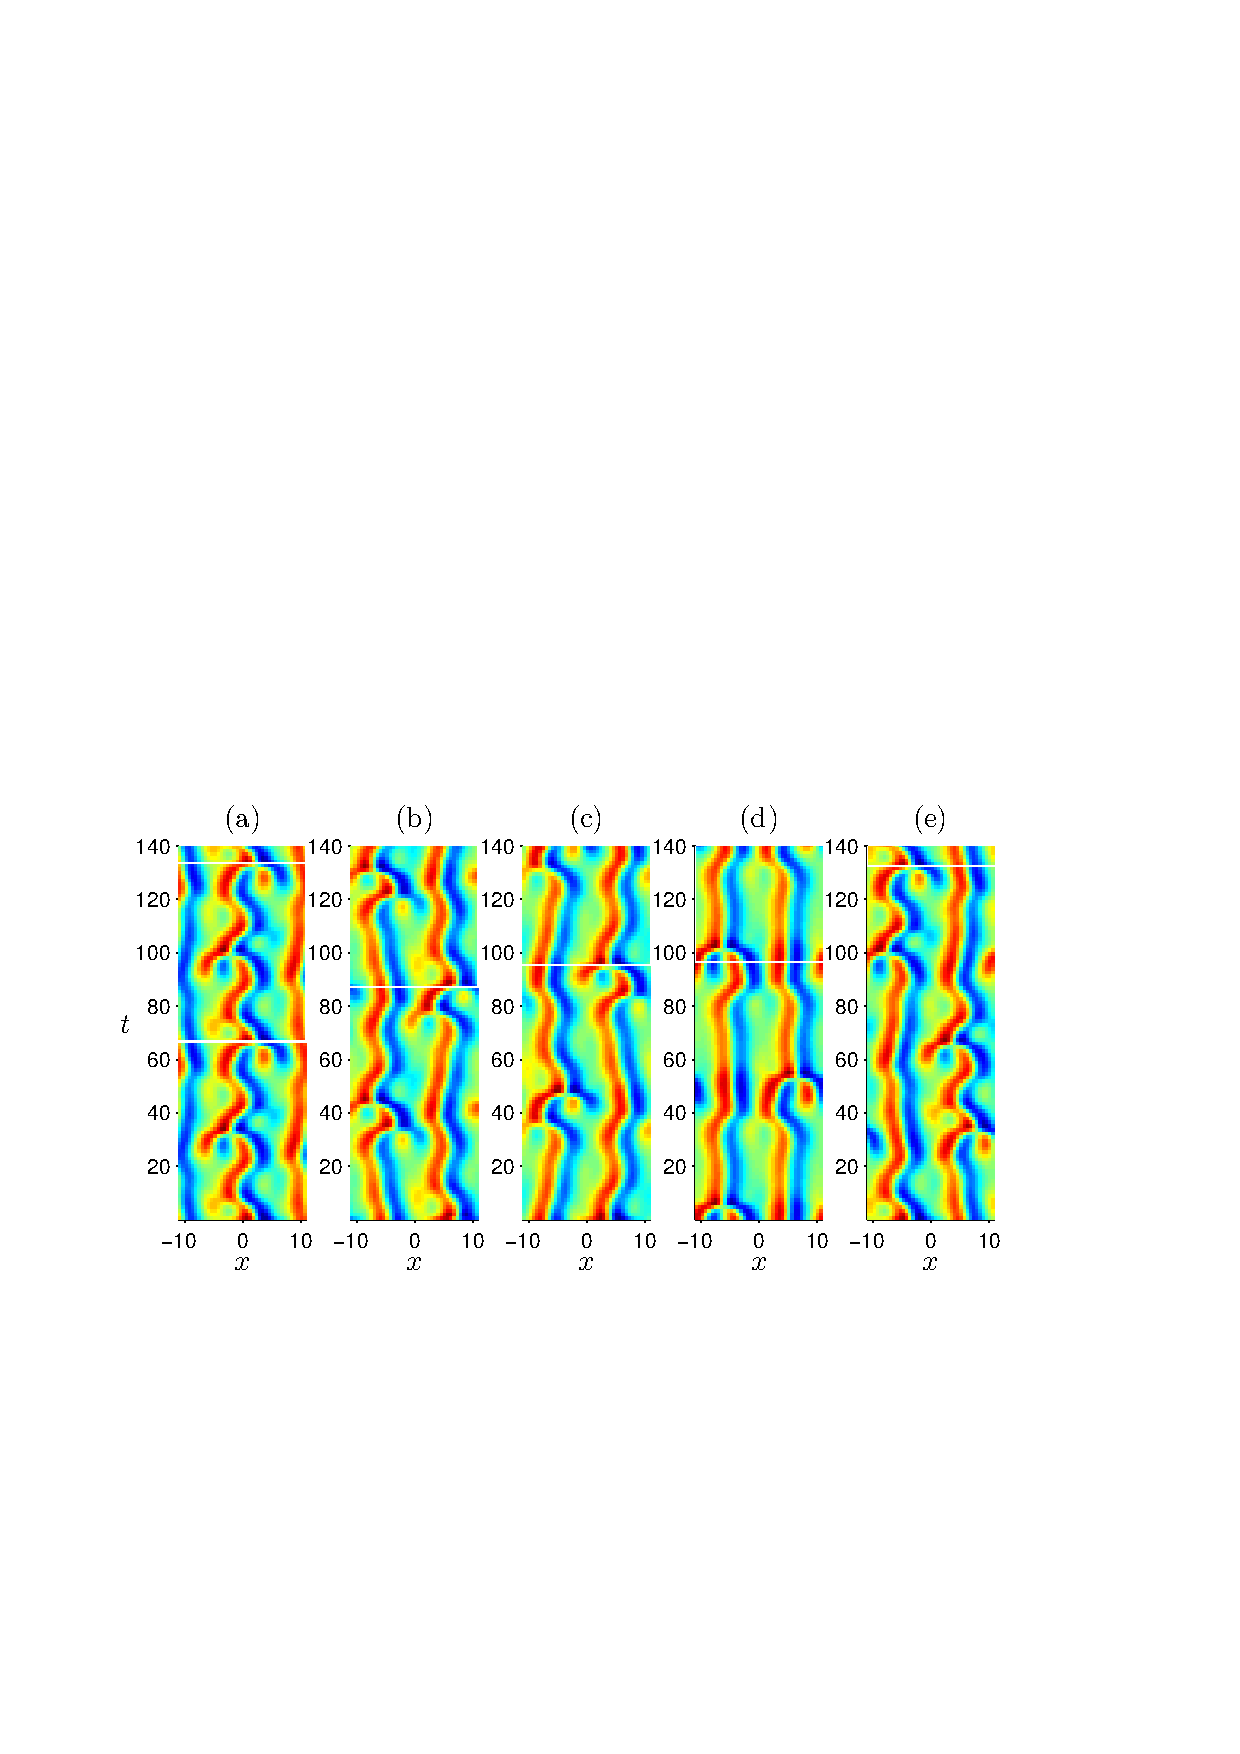
\includegraphics[width=0.9\textwidth]{figs/ks22rposPO}
%\begin{tabular}{ccccc} (a) & (b) & (c) & (d) & (e)\\
%$t$
%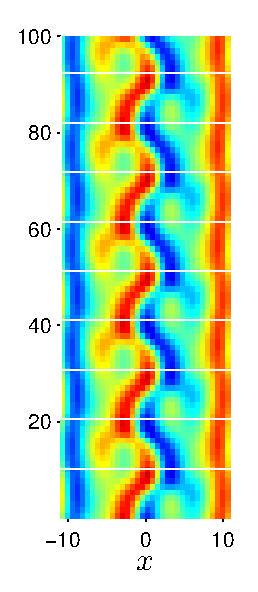
\includegraphics[width=0.18\textwidth]{figs/ks22rpo020.5-00.00}\hspace{-3ex} &
%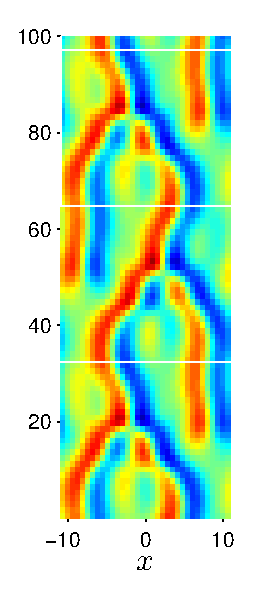
\includegraphics[width=0.18\textwidth]{figs/ks22rpo064.7-00.00}\hspace{-3ex} &
%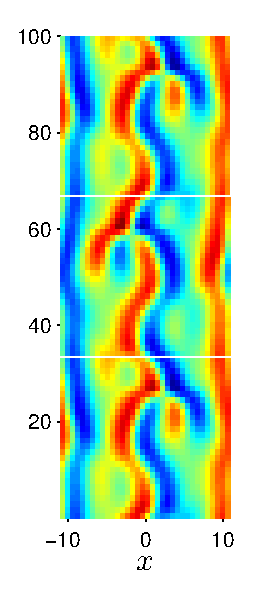
\includegraphics[width=0.18\textwidth]{figs/ks22rpo066.8-00.00}\hspace{-3ex} &
%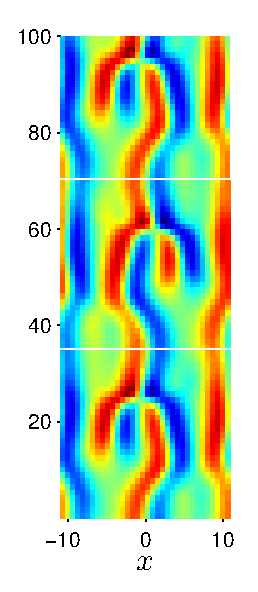
\includegraphics[width=0.18\textwidth]{figs/ks22rpo070.3-00.00}\hspace{-3ex} &
%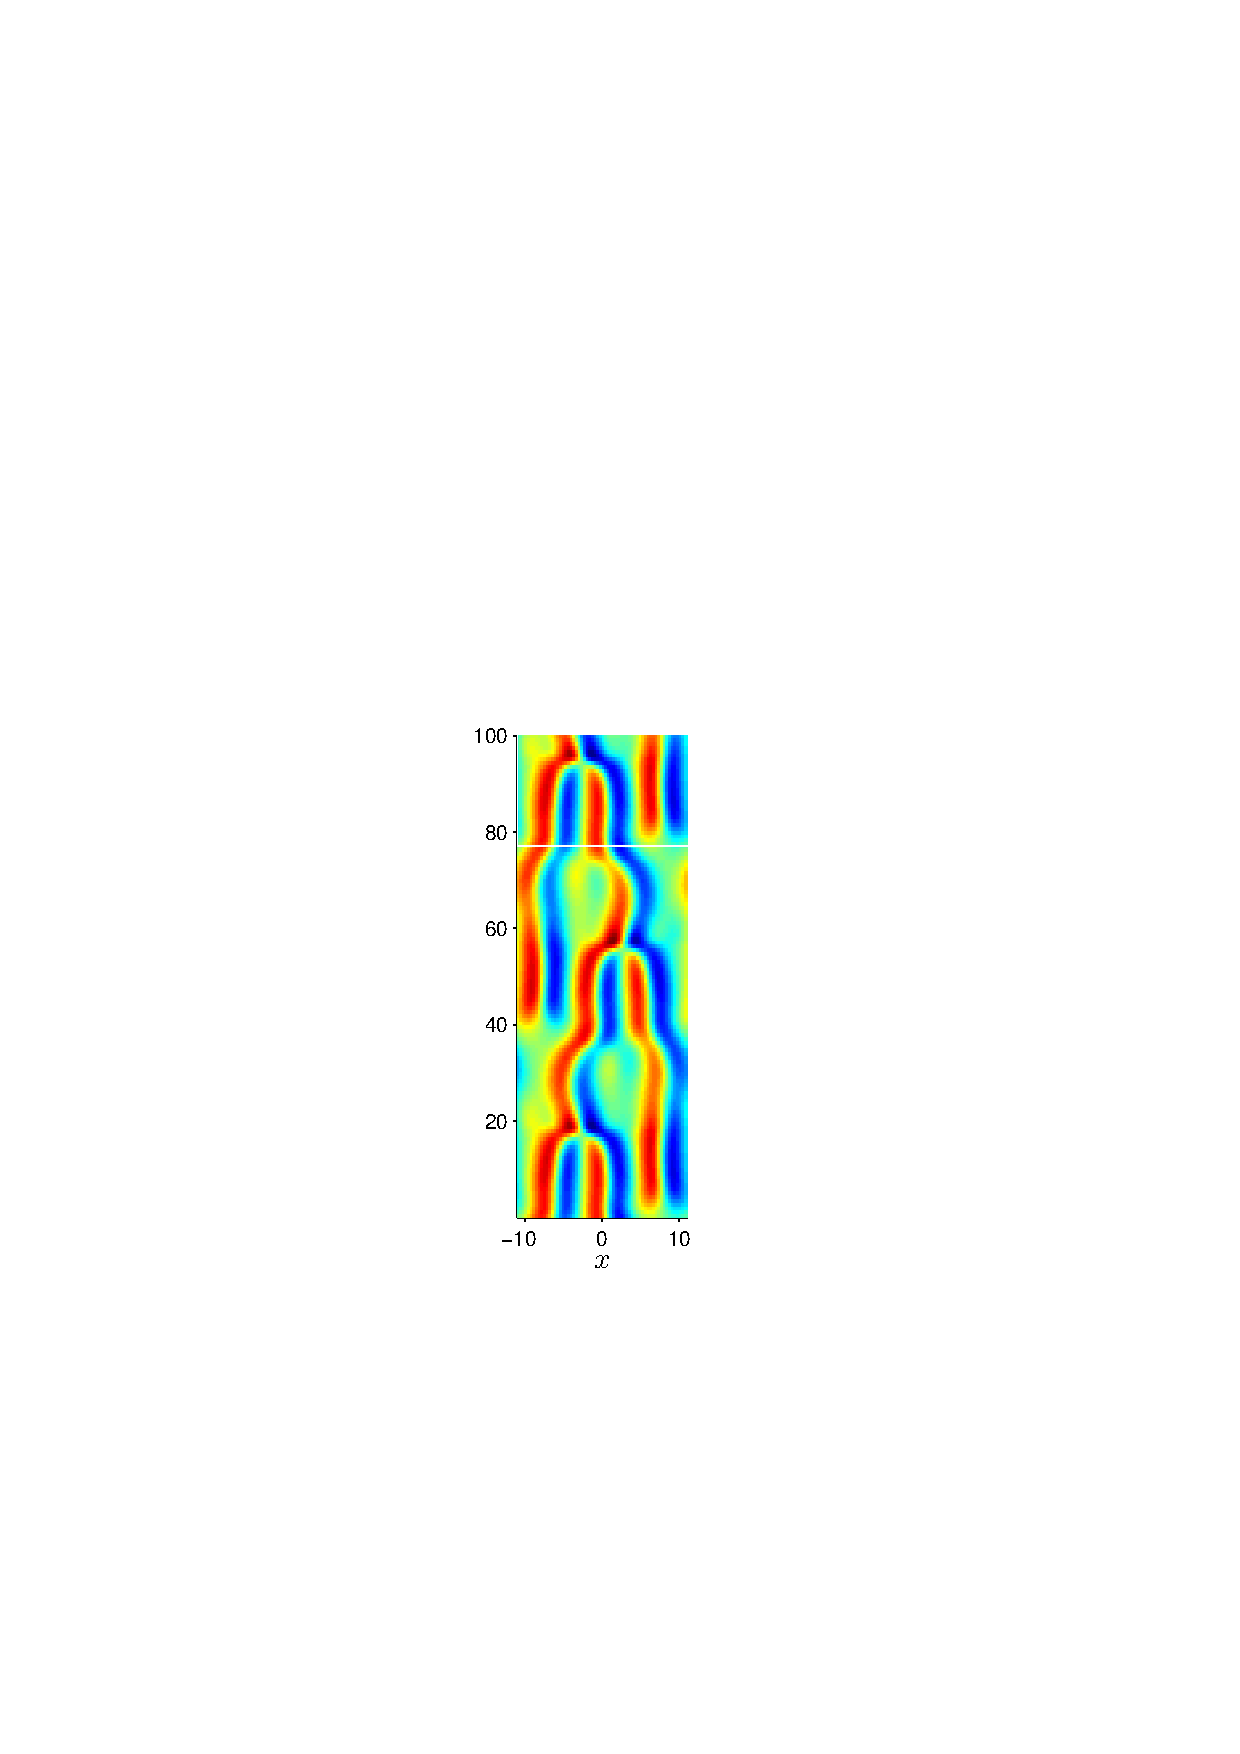
\includegraphics[width=0.18\textwidth]{figs/ks22rpo077.2-00.00}
%\end{tabular}
%\end{center}
%\caption{\Po s of \KS\ equation with $L = 22$:
%(a) $\period{} = 20.5$;
%(b) $\period{} = 64.7$;
%(a) $\period{} = 66.8$;
%(b) $\period{} = 70.3$;
%(c) $\period{} = 77.2$.} \label{f:ks22rposPO}

%\begin{figure}[t]
%\begin{center}
%%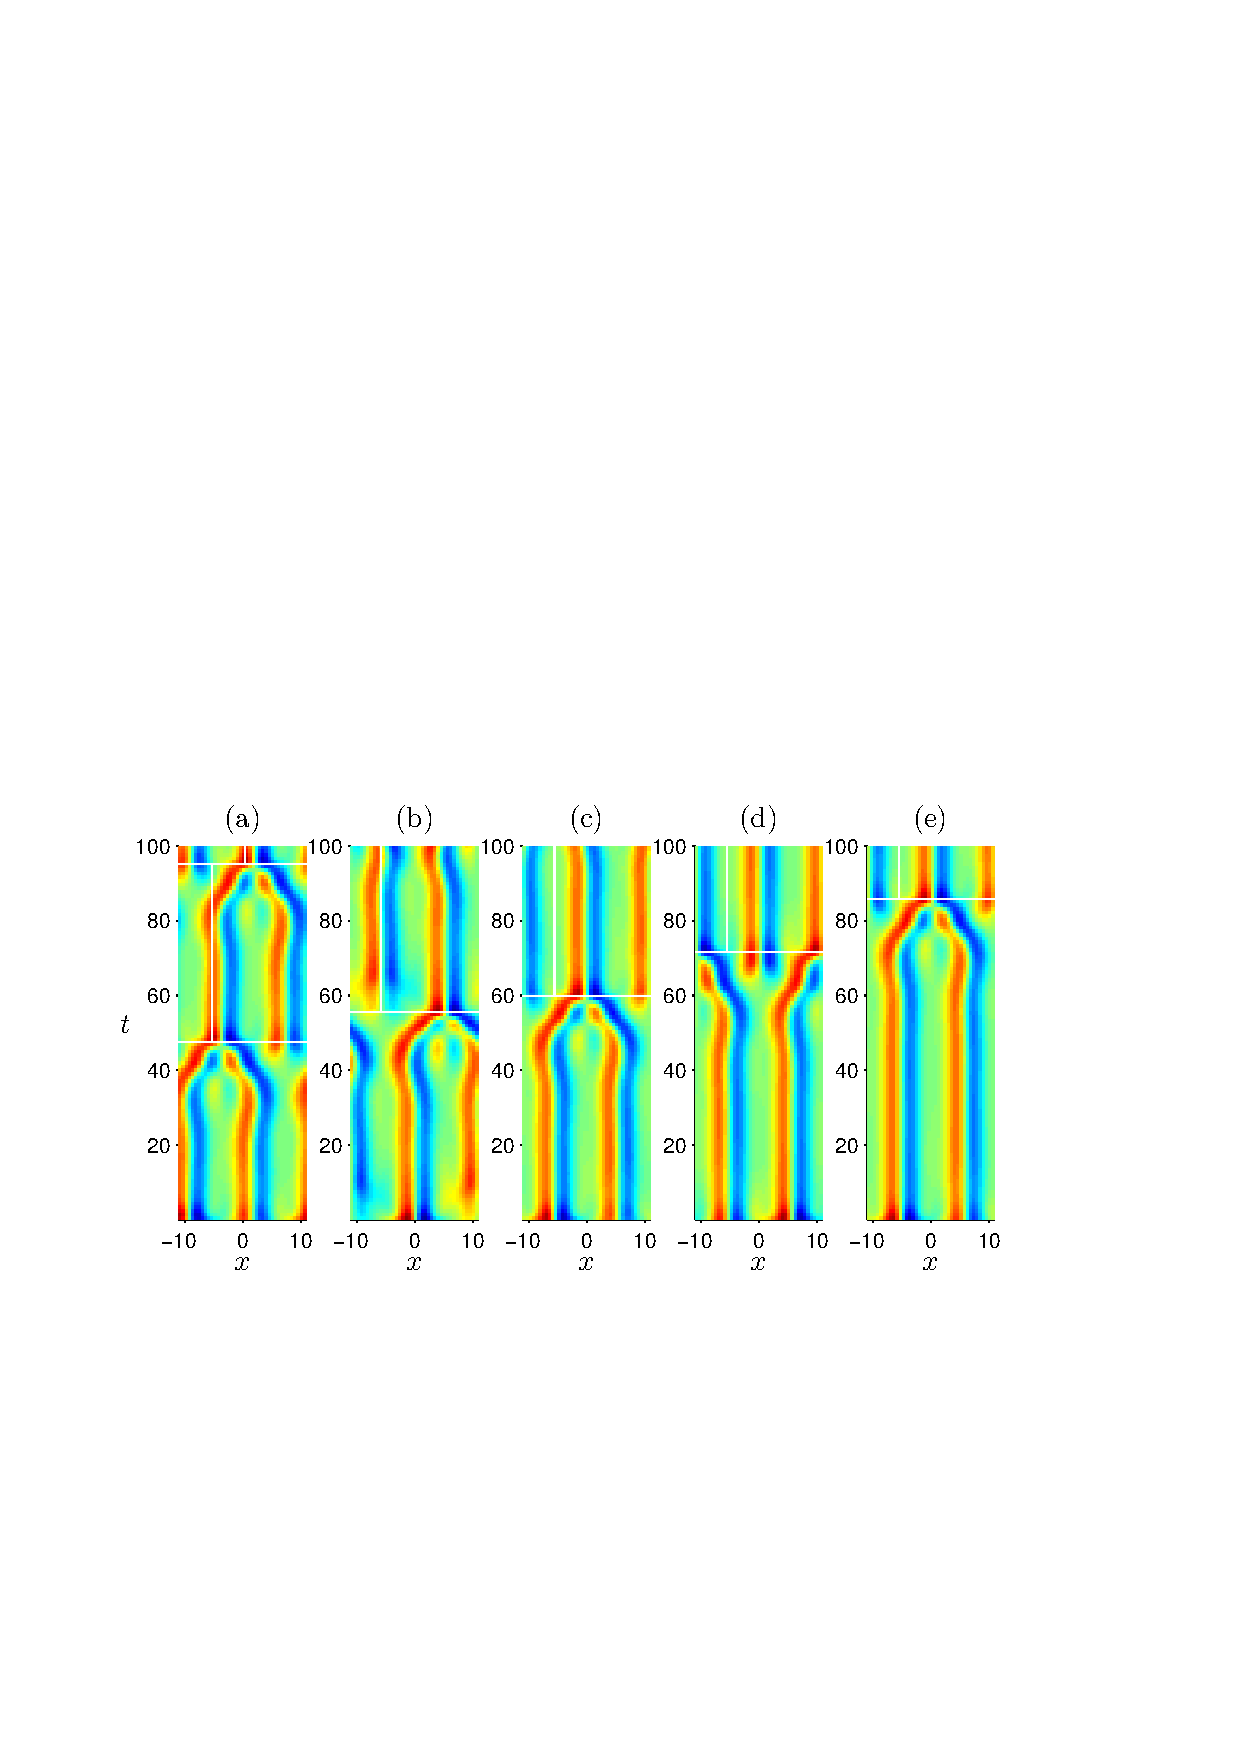
\includegraphics[width=0.9\textwidth]{figs/ks22rposCage}
%\begin{tabular}{ccccc} (a) & (b) & (c) & (d) & (e)\\
%$t$
%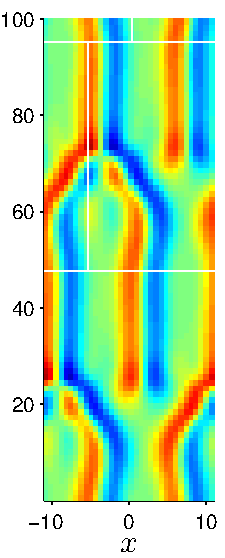
\includegraphics[width=0.18\textwidth]{figs/ks22rpo047.6-05.68}\hspace{-3ex} &
%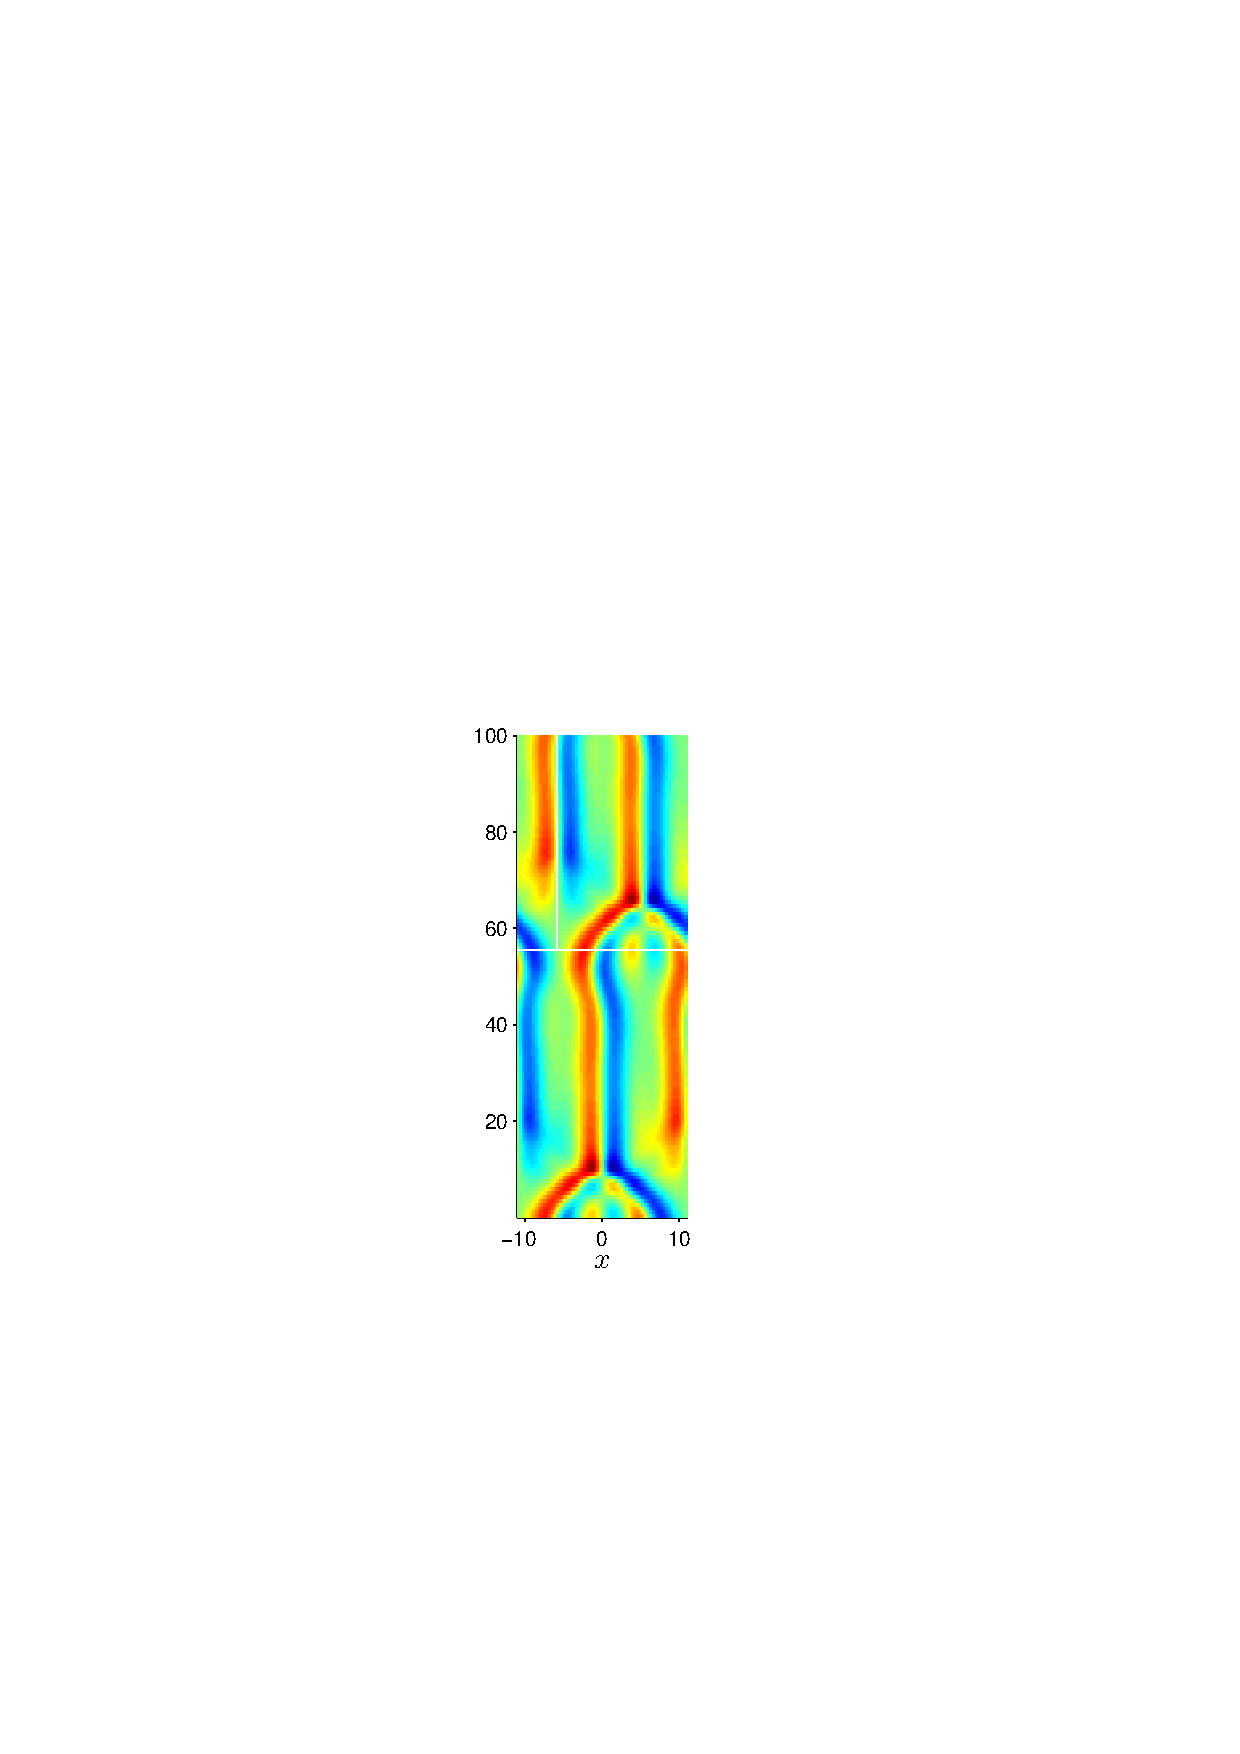
\includegraphics[width=0.18\textwidth]{figs/ks22rpo055.6-05.25}\hspace{-3ex} &
%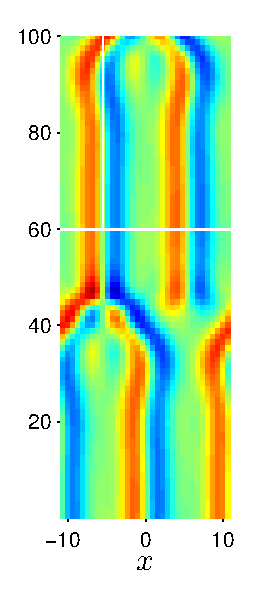
\includegraphics[width=0.18\textwidth]{figs/ks22rpo059.9-05.44}\hspace{-3ex} &
%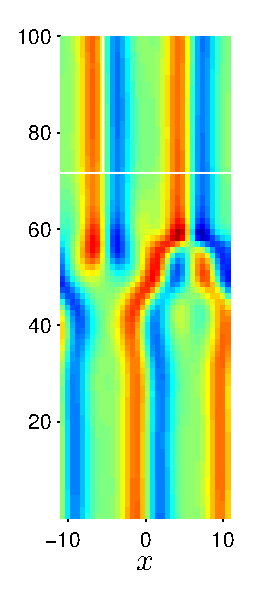
\includegraphics[width=0.18\textwidth]{figs/ks22rpo071.7-05.50}\hspace{-3ex} &
%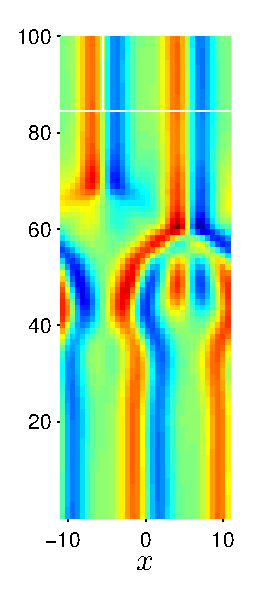
\includegraphics[width=0.18\textwidth]{figs/ks22rpo084.4-05.51}
%\end{tabular}
%\end{center}
%\caption{\Rpo s close to the unstable manifold of \EQV{2} \eqv.
%(a) $\period{} = 47.6$, $\shift = 5.68$;
%(b) $\period{} = 55.6$, $\shift = 5.25$;
%(c) $\period{} = 59.9$, $\shift = 5.44$;
%(d) $\period{} = 71.7$, $\shift = 5.503$;
%(e) $\period{} = 84.4$, $\shift = 5.513$.
%Horizontal and vertical white lines indicate periodicity and
%phase shift of the orbits, respectively. }\label{f:ks22rposCage}
%\end{figure}

%    \RLD{
%    \RLDedit{I've split the reffig~{f:ks22rposShort}
%plots and put them in the tabular,
%but I don't know how to place label $t$ to the left of the figures.
%Please fix this if you know how.  Otherwise I can include $t$ in the
%leftmost figure, but it will be a bit tricky since the aspect
%ratio of this figure will be different from the others.
%    }}
% \subsection{\Rpo s close to the unstable manifold of \EQV{2} }

% \PC{
%  Implementing Ruslan: all axes in reffig~{f:drivedragConn} changed by a factor
% of 2?
%         \\
% Implementing Predrag:
% label axes in reffig~{f:drivedrag}, reffig~{f:drivedragConn}
% by $(E,P,D,\dot{E})$
%     }
% \PC{ks22TurbConn2\_xfig for reffig~{f:drivedragConn}
%     not checked in?
%    }
% \PC{refFig~{f:drivedragConn}: split into three figures, \\
%     (a) label axes $(E,P)$, move to reffig~{f:drivedrag}\,(\textit{b})\\
%     (b) flip $y$ axis as $\dot{E}=P-D$; label axes $(P,\dot{E})$ \\
%     (c) flip $y$ axis; label axes $(E,\dot{E})$ \\
%    }

\medskip

RLD:{Replaced text: ``
As a result, KS equation can have
\rpo\ solutions with a profile $u_p(x)$, period $\period{p}$, and a
nonzero shift $\shift_p$, without or with reflection,
\begin{eqnarray}
  \Shift_{\shift_p/L}u(x,\period{p}) &=&
  u(x+\shift_p,\period{p}) = u(x,0) = u_p(x)\,,
\label{KSrpos0} \\
  \mbox{or} \quad \Refl\Shift_{\shift_p/L} u(x,\period{p}) &=&
  -u(-x-\shift_p,\period{p}) = u(x,0) = u_p(x)\,,
\label{KSpos0}
\end{eqnarray}
\ie, a profile $u(x,0) = u_p(x)$ that occurs again after time
$\period{p}$, but shifted by $\shift_p$, and possibly reflected by
$\Refl$.
   ''}
\RLD{
As a result, KS equation can have \rpo\ solutions with
a profile $u_p(x)$, period $\period{p}$, and a
nonzero shift $\shift_p$
\beq
  \Shift_{\shift_p/L}u(x+\shift,\period{p}) =
  u(x+\shift_p+\shift,\period{p}) = u(x+\shift,0) = u_p(x)\,,
\eeq
as well as \rpo s \emph{with reflection} which are characterized by
a profile $u_p(x)$ and a period $\period{p}$ and satisfy
the condition
\beq
  \Refl u(x+\shift,\period{p}) =
  -u(-x-\shift,\period{p}) = u(x+\shift,0) = u_p(x)
\label{KSpos1}
\eeq
with any $-L/2 < \shift \leq L/2$.
   } %end RLD

ES:{ I think we don't need the extra $\shift$. In the case with no reflection
the shift is uniquelly determined. In the case with reflection, since the term \rpo\
refers to the action of any group element under which the flow is invariant (not
necessarily translations) we can define this type of \rpo\ through
\[
  \Refl u(x,\period{p}) =
  -u(-x,\period{p}) = u(x,0) = u_p(x)\,.
\]
The \rpo s related to the action of $\Refl\Shift_{\shift/L}$ are equivalent (by translation) to
the last case (this is what Ruslan's footnote in refsect~{sec:L22} shows). Thus
there is no notion of shift associated with preperiodic orbits.
} %end ES

RLD:{
The reason I've introduced arbitrary $\shift$ is that this allows
the definition of the whole family of equivalent orbits related
by $\Shift_{\shift/L}$.  I agree with Vaggelis that, in case of \rpo s
without reflection, it makes no difference, since the condition
\refeq{KSrpos} remains true in any spatial reference frame.  So we could
drop $\shift$ here.

However, in the case of \po s (AKA \rpo s with reflection),
removing $\shift$ makes the condition \refeq{KSpos} valid only in
a specific reference frame, which is different for different \po s.
Hence the condition as written in \refeq{KSpos} cannot be used to
find \po s (i.e., you cannot derive \refeq{KSposFour} from it).

Now, if we don't use $\shift$ in \refeq{KSrpos}, but use it in \refeq{KSpos}
(like in \refeq{KSpos1}), then the two definitions are not equivalent,
since \refeq{KSrpos} defines just one orbit from the family related
by $\Shift_{\shift/L}$, while \refeq{KSpos1} defines the whole family.
   } %end RLD

ES:{ We can derive \refeq{KSposFour} by reversing Ruslan's proof:
applying $\Shift_{\shift/L}$ on \refeq{KSpos} we get
 $\Refl\Shift_{-2\shift/L}\left(\Shift_{\shift/L}u(x,T)\right)=\Shift_{\shift/L}u(x,0)\,,$
a condition for a \rpo\ of type \refeq{KSpos} in the translated frame, from which we get
\refeq{KSposFour}, to be used in practice since our initial guess might be translated
to another frame of reference.
The argument is that orbits of type \refeq{KSrpos} and \refeq{KSpos}
exist and are unique up to translational invariance.
We then can present the complications due to
translational invariance in their determination separately.
} %end ES


RLD:{
    The shift $\shift_p$ cannot be defined
    uniquely for a given pre-periodic orbit.  Let's say
    $\Refl\Shift_{\shift_p/L} u(x,\period{p}) = u(x,0)$.  The same
    orbit translated by any $\shift$ satisfies the condition
    $\Shift_{\shift/L}\Refl\Shift_{\shift_p/L} u(x,\period{p}) =
    \Shift_{\shift/L}u(x,0)$, or, since $\Shift_{\shift/L}\Refl = \Refl\Shift_{-\shift/L}$,
    this can be rewritten as follows:
    $\Refl\Shift_{(\shift_p - \shift)/L}u(x,\period{p}) =
    \Refl\Shift_{(\shift_p - 2\shift)/L}[\Shift_{\shift/L}u(x,\period{p})] =
    \Shift_{\shift/L}u(x,0)$, and so the new shift is now $\shift_p - 2\shift$.  Therefore
    $\shift_p$ can have any value depending on the spatial reference frame.  For example,
    we can always find a reference frame where $\shift_p = 0$ and thus the pre-periodic
    orbit satisfies the condition $u(x,\period{p}) = -u(-x,0)$.
    }

\begin{figure}[t]
\begin{center}
(\textit{a})\hspace{1ex}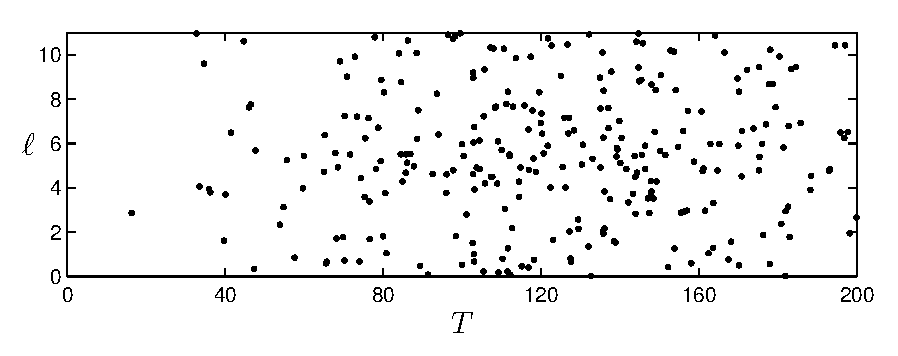
\includegraphics[width=0.7\textwidth, clip=true]
                            {ks22_rpos_Tdelta}\\
(\textit{b})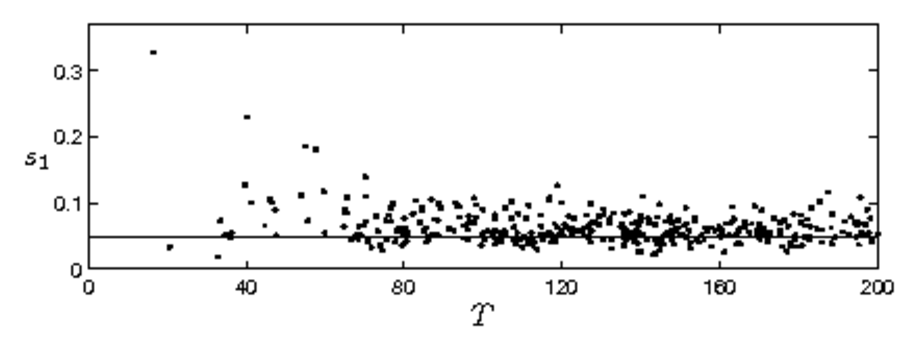
\includegraphics[width=0.72\textwidth, clip=true]
                            {ks22_rpos_lyap}
\end{center}
\caption{
(a) All \rpo s of \KSe\ determined here, with periods $\period{p}$ and
shifts $\shift_p > 0$.
(b) The largest Floquet exponents \refeq{FloqExp} of all
\rpo s and pre-periodic orbits with reflection.
The horizontal line at $0.048$
indicates the numerical value  of the largest
Lyapunov exponent of the chaotic attractor.
} \label{f:ks22rposT}
\end{figure}
